% ---------------------------------------------------------------------------------------------------------------
% TEMPLATE PARA TRABALHO DE CONCLUSÃO DE CURSO
% UEPG
% Customização da classe abnTeX2 (http://www.abntex.net.br/) para as normas da UEPG
%
% Projeto hospedado em: <link git>
%
%----------------------------------------------------------------------------------------------------------------
% Codificação: UTF-8
% LaTeX:  abnTeX2          
% ---------------------------------------------------------------------------------------------------------------


% CARREGA CLASSE PERSONALIZADA DA UEPG--------------------------------------------------------------------------
\documentclass[%twoside,                   % Impressão em frente e verso
    	        oneside,                   % Impressão apenas frente
]{config/uepg-abntex2}


% INCLUI ARQUIVOS DE CONFIGURAÇÕES-------------------------------------------------------------------------------
% REFERÊNCIAS------------------------------------------------------------------
\usepackage[%
    alf,
    abnt-emphasize=bf,
    bibjustif,
    recuo=0cm,
    abnt-url-package=url,       % Utiliza o pacote url
    abnt-refinfo=yes,           % Utiliza o estilo bibliográfico abnt-refinfo
    abnt-etal-cite=3,
    abnt-etal-list=3,
    abnt-thesis-year=final
]{abntex2cite}                  % Configura as citações bibliográficas conforme a norma ABNT

% PACOTES----------------------------------------------------------------------
\usepackage[utf8]{inputenc}                                 % Codificação do documento
\usepackage[T1]{fontenc}                                    % Seleção de código de fonte
\usepackage{booktabs}                                       % Réguas horizontais em tabelas
\usepackage{color, colortbl}                                % Controle das cores
\usepackage{float}                                          % Necessário para tabelas/figuras em ambiente multi-colunas
\usepackage{graphicx}                                       % Inclusão de gráficos e figuras
\usepackage{listings}                                       % Adicionar a listagem de código fonte

\lstset{ literate={á}{{\'a}}1 {ã}{{\~a}}1 {é}{{\'e}}1 {è}{{\`{e}}}1 {ê}{{\^{e}}}1 {ë}{{\¨{e}}}1 {É}{{\'{E}}}1 {Ê}{{\^{E}}}1 {û}{{\^{u}}}1 {ú}{{\'{u}}}1 {â}{{\^{a}}}1 {à}{{\`{a}}}1 {á}{{\'{a}}}1 {ã}{{\~{a}}}1 {Á}{{\'{A}}}1 {Â}{{\^{A}}}1 {Ã}{{\~{A}}}1 {ç}{{\c{c}}}1 {Ç}{{\c{C}}}1 {õ}{{\~{o}}}1 {ó}{{\'{o}}}1 {ô}{{\^{o}}}1 {Õ}{{\~{O}}}1 {Ó}{{\'{O}}}1 {Ô}{{\^{O}}}1 {î}{{\^{i}}}1 {Î}{{\^{I}}}1 {í}{{\'{i}}}1 {Í}{{\~{Í}}}1
}

\usepackage{xcolor}                                         % Adicionar cores personalizadas
\usepackage{icomma}                                         % Uso de vírgulas em expressões matemáticas
\usepackage{indentfirst}                                    % Indenta o primeiro parágrafo de cada seção
\usepackage{microtype}                                      % Melhora a justificação do documento
\usepackage{multirow, array}                                % Permite tabelas com múltiplas linhas e colunas
\usepackage{subeqnarray}                                    % Permite subnumeração de equações
\usepackage{lastpage}                                       % Para encontrar última página do documento
\usepackage{verbatim}                                       % Permite apresentar texto tal como escrito no documento, ainda que sejam comandos Latex
\usepackage{amsfonts, amssymb, amsmath}                     % Fontes e símbolos matemáticos
\usepackage[algoruled, portuguese]{algorithm2e}             % Permite escrever algoritmos em português
%\usepackage[scaled]{helvet}                                % Usa a fonte Helvetica
\usepackage{times}                                          % Usa a fonte Times
%\usepackage{newtxtext,newtxmath}
%\usepackage{palatino}                                      % Usa a fonte Palatino
%\usepackage{lmodern}                                       % Usa a fonte Latin Modern
\usepackage[bottom]{footmisc}                               % Mantém as notas de rodapé sempre na mesma posição
\usepackage{ae, aecompl}                                    % Fontes de alta qualidade
\usepackage{latexsym}                                       % Símbolos matemáticos
\usepackage{lscape}                                         % Permite páginas em modo "paisagem"
%\usepackage{picinpar}                                      % Dispor imagens em parágrafos
%\usepackage{scalefnt}                                      % Permite redimensionar tamanho da fonte
%\usepackage{subfig}                                        % Posicionamento de figuras
%\usepackage{upgreek}                                       % Fonte letras gregas
\usepackage[singlelinecheck=false,tableposition=bottom]{caption}
\usepackage{tabularx}
%\renewcommand*\familydefault{\sfdefault}
\usepackage{pdfpages}
\usepackage{csquotes}


% CONFIGURAÇÕES DE APARÊNCIA DO PDF FINAL--------------------------------------
\makeatletter
\hypersetup{%
    portuguese,
    colorlinks=true,   % true: "links" coloridos; false: "links" em caixas de texto
    linkcolor=black,    % Define cor dos "links" internos
    citecolor=black,    % Define cor dos "links" para as referências bibliográficas
    filecolor=black,    % Define cor dos "links" para arquivos
    urlcolor=blue,     % Define a cor dos "hiperlinks"
    breaklinks=true,
    pdftitle={\@title},
    pdfauthor={\@author},
    pdfkeywords={abnt, latex, abntex, abntex2}
}
\makeatother

% ALTERA O ASPECTO DA COR AZUL--------------------------------------------------
\definecolor{blue}{RGB}{41,5,195}

% REDEFINIÇÃO DE LABELS---------------------------------------------------------
\def\equationautorefname~#1\null{Equa\c c\~ao~(#1)\null}

% CRIA ÍNDICE REMISSIVO---------------------------------------------------------
\makeindex

% HIFENIZAÇÃO DE PALAVRAS QUE NÃO ESTÃO NO DICIONÁRIO---------------------------
\hyphenation{%
    qua-dros-cha-ve
    Kat-sa-gge-los
}



% INCLUI ARQUIVOS DO TRABALHO DE CONCLUSÃO DE CURSO (PRÉ-TEXTUAIS, TEXTUAIS, PÓS-TEXTUAIS)-----------------------

% INSERE CAPA E FOLHA DE ROSTO
% CAPA---------------------------------------------------------------------------------------------------

% ORIENTAÇÕES GERAIS-------------------------------------------------------------------------------------
% Caso algum dos campos não se aplique ao seu trabalho, como por exemplo,
% se não houve coorientador, apenas deixe vazio.
% Exemplos: 
% \coorientador{}
% \departamento{}

% DADOS DO TRABALHO--------------------------------------------------------------------------------------
\titulo{Testes automatizados aplicados no ciclo de vida de desenvolvimento de software: Estudo de caso da implementação em uma aplicação web}
\titleabstract{Title in English}
\autor{João Vitor Martins dos Santos}
\autorcitacao{Santos, João Vitor M.} % Sobrenome em maiúsculo
\local{Ponta Grossa}
\data{2022}

% NATUREZA DO TRABALHO-----------------------------------------------------------------------------------
% Opções: 
% - Trabalho de Conclusão de Curso (se for Graduação)
% - Dissertação (se for Mestrado)
% - Tese (se for Doutorado)
% - Projeto de Qualificação (se for Mestrado ou Doutorado)
\projeto{Trabalho de Conclusão de Curso}

% TÍTULO ACADÊMICO---------------------------------------------------------------------------------------
% Opções:
% - Bacharel ou Tecnólogo (Se a natureza for Trabalho de Conclusão de Curso)
% - Mestre (Se a natureza for Dissertação)
% - Doutor (Se a natureza for Tese)
% - Mestre ou Doutor (Se a natureza for Projeto de Qualificação)
\tituloAcademico{Bacharel em Engenharia de Software}

% ÁREA DE CONCENTRAÇÃO E LINHA DE PESQUISA---------------------------------------------------------------
% Se a natureza for Trabalho de Conclusão de Curso, deixe ambos os campos vazios
% Se for programa de Pós-graduação, indique a área de concentração e a linha de pesquisa
\areaconcentracao{}
\linhapesquisa{}

% DADOS DA INSTITUIÇÃO-----------------------------------------------------------------------------------
% Se a natureza for Trabalho de Conclusão de Curso, coloque o nome do curso de graduação em "programa"
% Formato para o logo da Instituição: \logoinstituicao{<escala>}{<caminho/nome do arquivo>}
\instituicao{Universidade Estadual de Ponta Grossa}
\setor{Setor de Engenharias, Ciências Agrárias e de Tecnologia}
\departamento{Departamento de Informática}
\programa{Curso de Engenharia de Software}
\logoinstituicao{0.2}{dados/figuras/uepg.png} 

% DADOS DOS ORIENTADORES---------------------------------------------------------------------------------
\orientador{Márcio Augusto de Souza}
%\orientador[Orientadora:]{Nome da orientadora}
\instOrientador{Universidade Estadual de Ponta Grossa}

\coorientador{Luiz Pedro Petroski}
%\coorientador[Coorientadora:]{Nome da coorientadora}
\instCoorientador{Pontifícia Universidade Católica do Paraná}

% FOLHA DE ROSTO--------------------------------------------------------------------------------------------------------

% TRABALHO DE CONCLUSÃO DE CURSO
 \preambulo{{\imprimirprojeto} no formato
 	de monografia apresentado ao {\imprimirdepartamento} - {\imprimirinstituicao}, como requisito para obtenção
 	do título de {\imprimirtituloAcademico}.}

% DISSERTAÇÃO DE MESTRADO
% \preambulo{{\imprimirprojeto} apresentada ao Programa de \mbox{Pós-graduação} da {\imprimirinstituicao}, como requisito parcial para obtenção do título de {\imprimirtituloAcademico}.}

% TESE DE DOUTORADO
% \preambulo{{\imprimirprojeto} apresentada ao Programa de \mbox{Pós-graduação} da {\imprimirinstituicao}, como requisito parcial para a obtenção do título de {\imprimirtituloAcademico}.}

% PROJETO DE QUALIFICAÇÃO DE MESTRADO OU DOUTORADO
%\preambulo{{\imprimirprojeto} apresentado ao Programa de \mbox{Pós-graduação} da {\imprimirinstituicao}, como requisito parcial para a obtenção do título de {\imprimirtituloAcademico}.}

% OBSERVAÇÕES-----------------------------------------------------------------------------------------------------------
% Altere este arquivo APENAS comentando as linhas que não se aplicam ao tipo de trabalho acadêmico desejado.



\begin{document}

\pretextual
\imprimircapa                                               	           % Comando para imprimir Capa
\imprimirfolhaderosto{}                                     		   % Comando para imprimir Folha de rosto
% INSERE ELEMENTOS PRÉ-TEXTUAIS
%% DEDICATÓRIA------------------------------------------------------------------

\renewcommand{\dedicatorianame}{DEDICATÓRIA}

\begin{dedicatoria}

Dedico aos meus pais, a minha noiva, a minha família, aos meus orientadores, a Júlio de Lima e a Rafael Sousa, meus mentores e irmãos pela fé em Cristo, a Thiago Teixeira e a Fábio Castro, meus amigos e aos meus colegas de profissão, testadores e analistas de qualidade.

%Observação: Para dedicatórias breves, recomenda-se o canto inferior direito, mas há liberdade para utilizar toda a folha.

\end{dedicatoria}
          			   % Dedicatória
%% AGRADECIMENTOS---------------------------------------------------------------

\begin{agradecimentos}[AGRADECIMENTOS]

A Deus por ter me sustentado e me dado condições de realizar esta monografia.

Ao Prof. Dr. Márcio Augusto de Souza e Prof. Me. Luiz Pedro Petroski por toda paciência, incentivos, contribuição com seus conhecimentos, revisões e sugestões na orientação desta monografia.

Ao meu amigo Thiago Teixeira que participa do desenvolvimento do software estudado nesta monografia.

Aos colegas de profissão que me colaboraram com suas opiniões e orientações.

Aos meus pais, a minha noiva e ao restante da minha família e aos amigos por acreditarem em mim.

A todos que direta ou indiretamente contribuíram para a conclusão desta pesquisa.

%Observação: No caso de vários agradecimentos, distribui-se proporcional/esteticamente o texto pelo espaço disponível na folha. Para um pequeno agradecimento, utiliza-se o canto inferior direito. Os agradecimentos devem ser feitos às pessoas e/ou instituições que contribuíram para a realização da pesquisa. Recomendam-se agradecimentos ao orientador, às pessoas envolvidas na pesquisa e às entidades financiadoras. 

\end{agradecimentos}
        			   % Agradecimentos
%% EPÍGRAFE---------------------------------------------------------------------

\renewcommand{\epigraphname}{EPÍGRAFE}

\begin{epigrafe}

\textit{Código sem testes é código ruim.\\
(Michael Feathers)}

\end{epigrafe}

% OBSERVAÇÕES------------------------------------------------------------------
% Altere o texto para inserir a epígrafe do seu trabalho

              			   % Epígrafe
% RESUMO--------------------------------------------------------------------------------

\begin{resumo}[RESUMO]
\begin{SingleSpacing}


Esta monografia apresenta uma proposta de um método para implementação de testes automatizados em projetos de software, utilizando como estudo de caso uma aplicação \emph{web} já desenvolvida e implementada utilizando o \emph{Framework web Laravel}, a qual foi desenvolvida sem a utilização de testes automatizados. Utilizaram-se procedimentos e técnicas encontrados na literatura para identificação e planejamento de testes para criar os cenários de testes de integração necessários para testar casos de uso da aplicação \emph{web} de forma eficaz. Foi proposta uma representação do sistema usando mapas mentais que permite visualizar os testes necessários mais facilmente. Esses testes foram automatizados utilizando a ferramenta \emph{PHPUnit}, configurada por padrão em projetos que utilizam o \emph{framewok Laravel}. Os testes foram executados, e seus resultados  analisados. A partir da análise dos resultados e das práticas utilizadas no planejamento dos testes e implementação dos \emph{scripts} propôs-se um conjunto de recomendações para implementação de testes automatizados.

\textbf{Palavras-chave}: Testes Automatizados. Testes de Integração. Qualidade de Software. \emph{Laravel}. \emph{PHPUnit}.

\end{SingleSpacing}
\end{resumo}

             			   % Resumo em Português
%% ABSTRACT--------------------------------------------------------------------------------

\begin{resumo}[ABSTRACT]
\begin{SingleSpacing}

This monograph has the objevtive to propose a method to automated test implementation in software projects, using as a case study an web application developed using the Laravel Framework and wich did not have automated tests. Using the procedures and test techniques found in the literature to identify tests, will be done the tests planning to identify the tests needed to verify the web application effectively, and then these tests will be automated using the PHPUnit and Laravel Dusk tools, provided by the Laravel Framework itself. Also will be build a continuous integration pipeline using Travis CI, in which the tests will be executed, then the execution results will be analysed. Based on these analisys, a set of best practices for automated tests implementation will be proposed. 

%Put your text here.\\

\textbf{Keywords}: Word. Second Word. Another word.

\end{SingleSpacing}
\end{resumo}

% OBSERVAÇÕES---------------------------------------------------------------------------
% Altere o texto inserindo o Abstract do seu trabalho.
% Escolha de 3 a 5 palavras ou termos que descrevam bem o seu trabalho 
             		           % Resumo em Inglês
% Lista de Figuras----------------------------------------------------------------

\pdfbookmark[0]{\listfigurename}{lof}
\listoffigures*
\cleardoublepage

% OBSERVAÇÕES---------------------------------------------------------------------
% Este arquivo não precisa de ser alterado, pois a lista é gerada automaticamente.
   % Lista de Figuras
%% LISTA DE QUADROS----------------------------------------------------------------

\renewcommand{\listofquadrosname}{LISTA DE QUADROS}

\pdfbookmark[0]{\listofquadrosname}{loq}
\listofquadros*
\cleardoublepage

% OBSERVAÇÕES---------------------------------------------------------------------
% Este arquivo não necessita de ser editado. A lista é gerada automaticamente.
   % Lista de Quadros
%% LISTA DE TABELAS-------------------------------------------------------------

\pdfbookmark[0]{\listtablename}{lot}
\listoftables*
\cleardoublepage

% OBSERVAÇÕES-------------------------------------------------------------------
% Este arquivo não precisa ser alterado, pois a lista é gerada automaticamente.
         		   % Lista de Tabelas
%% LISTA DE ABREVIATURAS E SIGLAS----------------------------------------------------------

\begin{siglas}
    \item[ABNT] Associação Brasileira de Normas Técnicas
    \item[DEINFO] Departamento de Informática
    \item[FTP] \textit{File Transfer Protocol}
    \item[HTTP] \textit{Hyper Text Transfer Protocol}
\end{siglas}

% OBSERVAÇÕES-----------------------------------------------------------------------------
% Altere a lista acima para definir os acrônimos e siglas utilizados neste trabalho
          		   % Lista de Abreviaturas e Siglas
%% LISTA DE SÍMBOLOS------------------------------------------------------------

\begin{simbolos}
    \item[$ \Gamma $] Letra grega Gama
    \item[$ \lambda $] Comprimento de onda
    \item[$ \in $] Pertence
\end{simbolos}

% OBSERVAÇÕES-------------------------------------------------------------------
% Altere a lista acima para definir os símbolos utilizados no trabalho
        		   % Lista de Símbolos
% LISTA DE ALGORITMOS----------------------------------------------------------

\newcommand{\algoritmoname}{Algoritmo}
%Definição de cores para listagem de algoritmos
\definecolor{codegreen}{rgb}{0,0.6,0}
\definecolor{codegray}{rgb}{0.5,0.5,0.5}
\definecolor{codepurple}{rgb}{0.58,0,0.82}
\definecolor{backcolour}{rgb}{0.95,0.95,0.92}

%Code listing style named "mystyle"
\lstdefinestyle{codigo}{
  backgroundcolor=\color{backcolour},   commentstyle=\color{codegreen},
  keywordstyle=\color{magenta},
  numberstyle=\tiny\color{codegray},
  stringstyle=\color{codepurple},
  basicstyle=\ttfamily\footnotesize,
  breakatwhitespace=false,         
  breaklines=true,                 
  captionpos=b,                    
  keepspaces=true,                 
  numbers=left,                    
  numbersep=5pt,                  
  showspaces=false,                
  showstringspaces=false,
  showtabs=false,                  
  tabsize=2
}
\renewcommand{\lstlistingname}{Algoritmo}
\renewcommand{\lstlistlistingname}{Lista de Algoritmos}

\lstset{style=codigo}

\lstlistoflistings
\cleardoublepage

% OBSERVAÇÕES------------------------------------------------------------------
% Este arquivo não precisa ser alterado, pois a lista é gerada automaticamente.
   % Lista de Algoritmos
% SUMÁRIO----------------------------------------------------------------------

\renewcommand{\contentsname}{SUMÁRIO}

\pdfbookmark[0]{\contentsname}{toc}
\tableofcontents*
\cleardoublepage

% OBSERVAÇÕES-------------------------------------------------------------------
% Este arquivo não precisa ser alterado, pois o sumário é gerado automaticamente.
               			   % Sumário

\textual
% INSERE ELEMENTOS TEXTUAIS
% INTRODUÇÃO-------------------------------------------------------------------

\chapter{INTRODUÇÃO}
\label{chap:introducao}

Softwares são suscetíveis a falhas em seu funcionamento, as quais são inconsistências entre o comportamento desejado do software e o comportamento apresentado pelo software desenvolvido. Essas falhas e inconsistências podem chegar até o usuário final, tendo potencial de gerar prejuízos à imagem do software e de seus responsáveis e até mesmo prejuízos financeiros. Entretanto a ausência de falhas não é a única característica de um software de qualidade, mas também abrange questões como a conformidade do comportamento do software com o que se propõe a fazer e até mesmo quão bem o software se comporta. Ou seja, além de estar livre de falhas o software deve atender as necessidades e expectativas de seus usuários. Dada a importância de se desenvolver software com qualidade, é fundamental que existam atividades de teste em projetos de desenvolvimento de software como forma de evitar que um software com baixa qualidade chegue ao usuário final.

Antes do surgimento do manifesto ágil, era comum que as atividades de teste de software fossem realizadas após o desenvolvimento do software ter sido finalizado. Além disso, geralmente os testes eram realizados de forma manual por equipes especializadas e dedicadas à realização de testes. 

Após o surgimento dos métodos ágeis, as atividades de teste passaram a ser mais valorizadas em qualquer tipo de software, e sofreram mudanças na forma como são executadas. Muitos testes passaram a ser automatizados, possibilitando que, além da detecção de erros, seja assegurado o correto funcionamento do software após alterações e também que os testes sirvam como documentação para o código desenvolvido. \cite{Valente2020}. Também é comum que as atividades de teste sejam realizadas pela própria equipe que realiza o desenvolvimento do software, não mais existindo fases e equipes dedicadas exclusivamente a realização de testes.

Para \citeonline{Crispin2009}, os testes manuais levam muito tempo e tendem a levar mais tempo a cada nova iteração, demandando que cada vez mais pessoas precisem dedicar tempo à realização de testes manuais, aumentando o débito técnico e a frustração. Os testes automatizados fornecem \emph{feedback} rapidamente e frequentemente, através da execução de testes sempre que há escrita de código novo. Erros causados por alterações no comportamento do software devido às mudanças do código podem ser detectados, possibilitando que as correções ocorram rapidamente. A automação de testes proporciona a redução do tempo necessário para execução dos testes de um software quando ele sofre atualizações, além da criação automática de relatórios sobre a execução dos testes automatizados.

É consenso entre os profissionais que desenvolvem software que é necessário testar o código desenvolvido, mas  as atividades de escrita de código de testes são frequentemente deixadas de lado devido à urgência e à pressão para terminar um projeto. Quanto maior a urgência e a pressão, menos testes são escritos. Escrevendo menos testes a produtividade diminui, pois o código torna-se menos estável. Consequentemente, com menor produtividade, a urgência e a pressão aumentam, alimentando um ciclo que leva os profissionais a exaustão. A melhor forma de persuasão sobre o valor da criação de \emph{scripts} de teste é implementando os testes em um projeto de desenvolvimento real, mostrando na prática o real valor do \emph{feedback} rápido fornecido pela execução dos testes e os benefícios que oferecem para a refatoração de código \cite{beck1998test}.

A criação dos \emph{scripts} de testes automatizados demanda tempo, mas os benefícios de sua implementação geram redução de tempo em outras atividades do projeto, como a execução dos testes, economizando cada vez mais tempo e esforço a longo prazo. Entretanto para implementar testes automatizados são necessários conhecimentos sobre planejamento de testes, codificação e ferramentas para criação e execução de \emph{scripts} de testes automatizados.

Dito isso é de importante estudar a implementação de testes automatizados em projetos reais de desenvolvimento de software, buscando explorar as práticas necessárias para implementação dos mesmos, além dos benefícios e as dificuldades enfrentadas para sua implementação. Este trabalho se propõe a realizar tal estudo com intuito de fornecer recomendações para a implementação de testes automatizados, dados seus benefícios e importância.

\section{OBJETIVO GERAL}

O objetivo deste trabalho é propor um método para implementação de testes automatizados em projetos de software.

\section{OBJETIVOS ESPECÍFICOS}
Com base no objetivo geral, foram definidos objetivos específicos:

\begin{itemize}
    \item Buscar na literatura processos de realização de teste de software e implementação de testes automatizados;
    \item Definir uma forma de representação dos cenários de teste baseada em mapas mentais para facilitar a definição dos testes a serem feitos;
    \item Inserir o processo de testes no fluxo de trabalho de métodos ágeis;
    \item Apresentar um estudo de caso do uso de testes em um software desenvolvido anteriormente chamado Sistema Admink;
    \item Definir um conjunto de recomendações para aplicação de testes automatizados de integração.
    
\end{itemize}

\section{ORGANIZAÇÃO DO TEXTO}
O texto deste trabalho está disposto da seguinte forma:
\begin{itemize}
    \item \autoref{chap:processos-de-software}: Aborda os processos de produção de software, suas características e evolução ao longo do tempo;
    \item \autoref{chap:teste-de-software}: Descreve conceitos e práticas de teste de software e testes automatizados;
    \item \autoref{chap:metodologia}: Detalha o material e os métodos utilizados na implementação de testes automatizados neste estudo;
    \item \autoref{chap:resultados}: Mostra os resultados obtidos após a implementação e execução dos testes automatizados e as recomendações propostas;
    \item \autoref{chap:conclusao}: Explora as conclusões alcançadas.
\end{itemize}                		           % Introdução
% REVISÃO DE LITERATURA--------------------------------------------------------
\chapter{PROCESSO DE DESENVOLVIMENTO DE SOFTWARE}
\label{chap:processos-de-software}

Para que equipes produzam software com qualidade e de forma produtiva é necessário um ordenamento mesmo que mínimo. O processo de desenvolvimento de software determina um conjunto de ações que devem ser seguidas. Seu uso é importante para que as empresas possam gerenciar o trabalho de produção de software garantindo a produtividade e o alinhamento com os objetivos da empresa. Também é importante para os desenvolvedores, para que estejam cientes de suas tarefas e dos resultados esperados e para que não se sintam perdidos, desalinhados com os demais envolvidos ou para que não trabalhem sem previsibilidade \cite{Valente2020}.

Neste capítulo serão abordadas duas alternativas distintas de processos de desenvolvimento de software, começando pelos processos tradicionais, com foco nas características do Modelo Cascata, um dos primeiros processos criados para desenvolvimento de software, o qual é baseado em processo da Engenharia tradicional. Em seguida serão abordados os processos ágeis, que foram propostos como alternativa aos processos tradicionais por um grupo de profissionais insatisfeitos que buscavam resolver os principais problemas dos processos utilizados até então, com foco nas características do método de Programação Extrema, conhecido como XP.

Os termos processos, métodos e modelos são utilizados neste trabalho como sinônimos para se referir ao conjunto de atividades e práticas utilizadas no desenvolvimento de software.

    \section{PROCESSOS SEQUENCIAIS}
    Os processos sequenciais de desenvolvimento de software surgiram baseados em projetos de Engenharia tradicional, como a engenharia eletrônica e engenharia civil, nos quais existem planejamentos detalhados previamente e etapas sequenciais que geram documentações detalhadas em cada etapa do processo \cite{Valente2020}.
    
    O ciclo de vida clássico de desenvolvimento de software, conhecido como Modelo Cascata \cite{Pressman2015}, propõe uma abordagem de fases sequenciais (\autoref{fig:modelo-cascata}). 
    
    \begin{figure}[!htb]
	    \centering
	    \sbox0{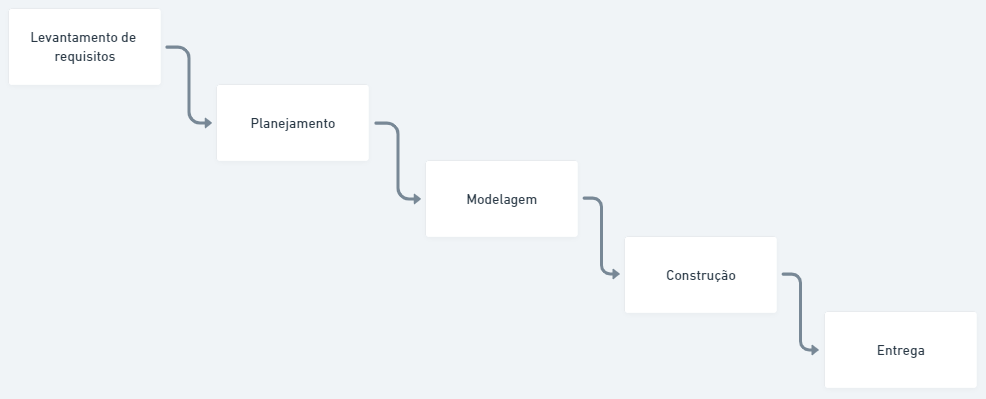
\includegraphics[width=1\textwidth]{./assets/figuras/ModeloCascata}}% measure width
	    \begin{minipage}{\wd0}
		    \usebox0
		    \caption{Fases do Modelo Cascata}
		    \label{fig:modelo-cascata}
		    \fonte{\citeonline{Pressman2015}}
	    \end{minipage}
    \end{figure}
    
    As fases podem  durar semanas ou meses e a fase seguinte só é iniciada após a fase anterior ter sido finalizada. Cada fase possui foco e atividades específicas:
        \begin{itemize}
            \item O projeto inicia com a fase de levantamento dos requisitos, na qual são realizadas atividades para identificação das necessidades do cliente do projeto;
            \item Em seguida ocorre a fase de planejamento, incluindo atividades de estimativas, cronograma e acompanhamento;
            \item O projeto avança pela fase de modelagem, na qual são realizadas a análise, o projeto do software e a construção de diagramas e modelos;
            \item Na sequência ocorre a fase de construção do software, a qual engloba as atividades de codificação e em seguida os testes do software;
            \item Por fim o projeto chega na fase final, na qual é realizada a entrega do software, é prestado suporte e são obtidos os \emph{feedbacks} do cliente.
            
        \end{itemize}
        
    As atividades de garantia de qualidade e de testes executadas na fase de construção se relacionam com o que é produzido nas fases anteriores. O modelo V (\autoref{fig:modelo-v})  é uma representação de quais atividades de teste estão relacionadas com os trabalhos de cada uma das fases do projeto. \cite{Pressman2015}
    
    \begin{figure}[!htb]
	    \centering
	    \sbox0{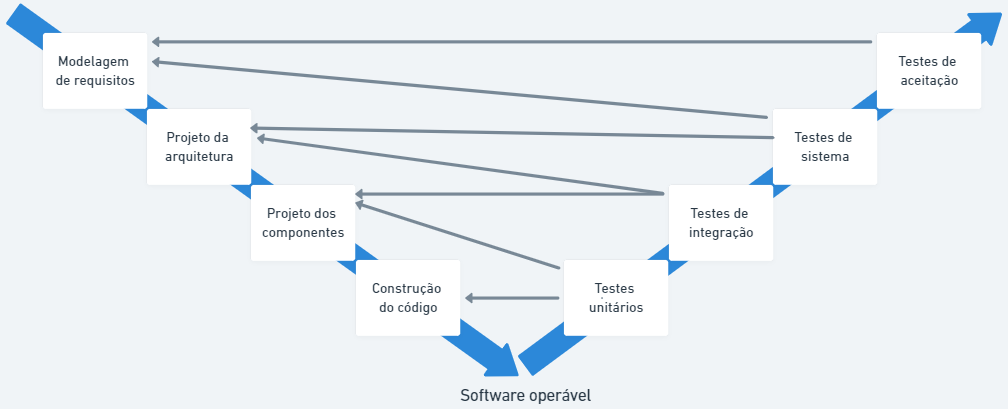
\includegraphics[width=1\textwidth]{./assets/figuras/ModeloV}}% measure width
	    \begin{minipage}{\wd0}
		    \usebox0
		    \caption{Modelo V}
		    \label{fig:modelo-v}
		    \fonte{\citeonline{Pressman2015}}
	    \end{minipage}
    \end{figure}
   
    As atividades de testes em processos sequenciais como o Cascata geralmente são realizadas manualmente por equipes dedicadas à execução de testes e ocorrem após finalizado o desenvolvimento do software. O software, que já está maduro o suficiente para ser executado, é utilizado nos testes de forma semelhante a que será utilizado pelos usuários finais, mas são informados dados de entrada específicos para teste. Os testes obtêm sucesso quando os comportamentos apresentados pelo software após a realização dos testes estiverem de acordo com aos comportamentos que são esperados que sejam apresentados, com base nas especificações produzidas nas fases anteriores e atendendo às necessidades dos usuários. 
    
    Como um dos objetivos das atividades de teste é o de revelar defeitos do software, a realização dos testes traz à tona erros cometidos em fases anteriores à de testes, como codificações incorretas, as quais causam falhas durante a execução ou comportamentos inconsistentes. Quanto mais tarde os defeitos forem encontrados, mais onerosa será a correção, pois além da correção do código do software para que não apresente mais tal defeito, poderá ser necessária a adequação da documentação produzida para que corresponda às alterações realizadas no software para corrigir o defeito.
    
    Testes de software tem relação direta com o processo de desenvolvimento de software, apresentando diversos conceitos e definições que serão exploradas no \autoref{chap:teste-de-software} com maior profundidade.
    
    O modelo cascata pode ser considerado o primeiro processo de desenvolvimento de software, mas ao longo dos anos sua eficácia passou a ser questionada. Alguns dos problemas encontrados são \cite{Pressman2015}:
        
        \begin{itemize}
            \item Os projetos reais raramente seguem um fluxo linear e sequencial, então as mudanças podem ocasionar confusão à medida que o projeto avança;
            \item Geralmente o cliente tem dificuldade de explicitar todas as suas necessidades no início do projeto, como é requerido pelo modelo cascata;
            \item As versões operáveis do software só estarão disponíveis próximos ao final do projeto, ocasionando em uma tardia detecção de erros e em descontentamentos do cliente.
        \end{itemize}
        
    Os processos sequenciais podem funcionar bem para projetos que possuem requisitos fixos e nos quais o projeto pode ser executado do começo ao fim de forma linear sem muitas mudanças, de maneira que são recomendados para projetos com incertezas ou mudanças frequentes o uso de processos ágeis.
    
    \section{PROCESSOS ÁGEIS}
    
    Devido aos problemas dos processos tradicionais, um grupo de profissionais se reuniu para propor uma alternativa ao processos sequenciais para desenvolvimento de software, defendendo que software é diferente de produtos tradicionais da Engenharia, portanto necessita de um processo de desenvolvimento diferente. Esse encontro resultou em um documento que é conhecido como manifesto ágil. Com o manifesto ágil passam a ser valorizados \cite{Valente2020}:
    \begin{itemize}
        \item Indivíduos e interações, mais do que processos e ferramentas;
        \item Validação do software mais do que uma documentação abrangente;
        \item Colaboração com o cliente mais do que negociação de contratos;
        \item Responder a mudanças mais do que seguir um plano.
    \end{itemize}
    
    O que caracteriza os processos ágeis são os ciclos de desenvolvimento iterativos e de curta duração, de uma a quatro semanas. O sistema é implementado gradualmente, começando pela implementação de uma versão com as funcionalidades que são mais prioritárias para o cliente. Após o cliente validar e aprovar essa versão, um novo ciclo, também chamado de iteração, é iniciado dando sequência ao desenvolvimento das demais funcionalidades também priorizadas pelo cliente, de maneira que todo ciclo produz uma versão funcional do software. O desenvolvimento é finalizado quando o cliente entende que todas as funcionalidades estão implementadas \cite{Valente2020}.
    
    Além dos valores do manifesto ágil, há 12 princípios de agilidade \cite{Pressman2015}:
    \begin{itemize}
        \item A maior prioridade é satisfazer o cliente através da entrega antecipada e contínua de software de valor;
        \item Mudanças nos requisitos são bem-vindas mesmo no fim do desenvolvimento, pois os processos ágeis aproveitam as mudanças como vantagem competitiva para o cliente;
        \item Deve-se entregar software funcionando frequentemente, de algumas semanas a alguns meses, preferindo-se os intervalos mais curtos;
        \item Pessoas de negócio e desenvolvedores devem trabalhar juntos diariamente ao longo do projeto;
        \item Deve-se construir projetos em torno de indivíduos motivados, dando a eles o ambiente e o suporte que precisarem, confiando neles para fazer o trabalho;
        \item O método mais eficiente e efetivo de transmitir informações com a equipe de desenvolvimento é a conversa cara a cara;
        \item Software funcionando é a principal medida de progresso;
        \item Processos ágeis promovem desenvolvimento sustentável. Os patrocinadores, desenvolvedores e usuários devem ser capaz de manter um ritmo constante indefinidamente;
        \item Atenção contínua para excelência técnica e bom projeto (\emph{design}) eleva a agilidade;
        \item Simplicidade, a arte da maximização do trabalho economizado, é essencial;
        \item As melhores arquiteturas, requisitos e projetos emergem de equipes auto-organizadas.
        \item Regularmente a equipe reflete sobre como se tornar mais efetiva, então sintoniza e ajusta seu comportamento de acordo.
    \end{itemize}
    
    Os processos que aplicam os valores e princípios do manifesto ágil mudam a visão sobre a responsabilidade pelas atividades de validação e testes. Todo time torna-se responsável por tais atividades e pela qualidade do software produzido, não sendo mais uma responsabilidade exclusiva de uma equipe de testes diferente da que realiza o desenvolvimento.
    
    Algumas outras características dos processos ágeis são: documentação apenas do que é essencial, sendo mais importante conseguir avançar mesmo com incertezas e possibilidade de mudança do que fazer um plano detalhado; não existência de uma fase dedicada ao projeto (\emph{design}), o qual também é feito de forma incremental; organização de times pequenos de desenvolvimento; e ênfase em novas práticas de desenvolvimento como programação em pares, testes automatizados e integração contínua. Devido a essas características, os processos ágeis são considerados leves, com pouca documentação. Essas características são genéricas e abrangentes, então foram criados métodos para auxiliar na adoção dos valores e princípios ágeis de forma concreta. \cite{Valente2020}. 
    
    Apesar de haver diversos métodos que aplicam os valores e princípios do manifesto ágil, neste trabalho será abordado o método intitulado Programação Extrema (\emph{Extreme Programming}), também conhecido como XP. O método XP é um dos mais bem definidos e completos e é o mais recomendado para entender a metodologia ágil, pois outros métodos ágeis empregam subconjuntos ou variações do XP, além de empregar práticas de testes automatizados em seu ciclo de vida \cite{Martin2020}, que são o foco deste trabalho.
        
        \subsection{Programação Extrema (XP)}
        
        O XP é um método leve recomendado para o desenvolvimento de software com requisitos imprecisos ou sujeitos a mudança e aplica as características dos processos ágeis. Entretanto o XP não define uma sequência detalhada de passos para produzir software, e sim um conjunto de valores e princípios que devem fazer parte da cultura e do dia a dia dos times de desenvolvimento, então esses valores e princípios são concretizados em práticas de desenvolvimento \cite{Valente2020}.
        
        O XP é conduzido pelos valores da comunicação, simplicidade, \emph{feedback}, coragem e respeito. Boa comunicação é essencial para evitar erros e também aprender com eles. A simplicidade é importante para focar em projetar mais as necessidades atuais que as futuras, produzindo projetos fáceis de serem implementados e que podem ser evoluídos futuramente, caso necessário. O rápido \emph{feedback} do cliente, dos membros da equipe e do próprio software através de uma estratégia de testes eficaz são essenciais para controlar riscos e diminuir prejuízos e retrabalhos. É necessário ter coragem e disciplina para projetar para as necessidades atuais, tendo em mente que as necessidades futuras podem mudar e exigir mudanças no projeto e no código. Os integrantes de time ágeis devem respeitar os demais membros da equipe, os demais envolvidos no projeto, o próprio software, além de ter respeito pelo processo XP \cite{Pressman2015}.
        
        A aplicação dos valores de simplicidade, comunicação e o \emph{feedback} representado pelos testes proporcionam um avanço mútuo, pois um valor beneficia o outro:  Os testes melhoram a comunicação através do registro das interfaces do programa; A comunicação melhora os testes aumentando as chances de defeitos serem revelados; A simplicidade é aumentada pelos testes, pois aumentam a possibilidade de refatorar código facilmente; E a simplicidade melhora os testes, pois um código mais simples é mais simples de se testar (\cite{beck1998}).
        
        Além desses valores, o XP também possui alguns princípios que são procedimentos mais concretos e pragmáticos \cite{Valente2020}:
        \begin{itemize}
            \item Humanidade: O principal recurso de uma empresa são seus colaboradores. Uma boa gestão de pessoas é a chave para o sucesso de projetos de software;
            \item Economicidade: Software é caro e quem está pagando por ele espera resultados econômicos e financeiros, então software não é uma obra de arte, mas uma produção que precisa de resultados econômicos;
            \item Benefícios Mútuos: As decisões tomadas nos projetos de software devem beneficiar a múltiplos envolvidos;
            \item Melhorias Contínuas: Como nenhum processo de desenvolvimento de software é perfeito, trabalhar em um software e em práticas de desenvolvimento que são aprimoradas a cada iteração a partir \emph{feedback} do cliente e da equipe é mais seguro;
            \item Falhas Acontecem: Software é uma das construções humanas mais complexas, então é esperado que softwares apresentem falhas e inconsistências. Elas não devem ser encobertas, mas também não devem ser usadas para punição do time;
            \item Passos de bebê (\emph{baby steps}): Pequenos progressos contínuos na direção certa são melhores que grandes revoluções, pois estas costumam gerar resultados negativos. Ou seja, é melhor concluir pequenas atividades constantemente que acumular uma grande quantidade de trabalho realizado aguardando ser concluído;
            \item Responsabilidade Pessoal: Os desenvolvedores devem ter clareza de seu papel e responsabilidade na equipe. O engenheiro de software que realiza a implementação também é responsável pelos testes e manutenção.
        \end{itemize}
        
        Além dos valores e princípios, o XP adota um conjunto de práticas para desenvolvimento ágil de software conhecidas como Ciclo de Vida. Muitas dessas práticas podem ser aplicadas inclusive em projetos que utilizam outros métodos ágeis. Algumas das práticas são orientadas para os negócios, outras para a equipe e outras são práticas técnicas (\autoref{fig:cicloXP}).
        
        \begin{figure}[!htb]
	        \centering
	        \sbox0{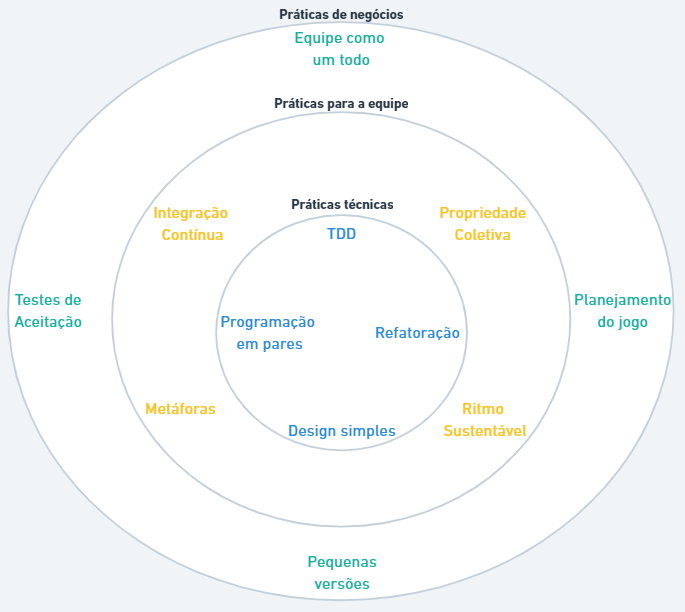
\includegraphics[width=1\textwidth]{./assets/figuras/CicloXP}}% measure width
	        \begin{minipage}{\wd0}
		        \usebox0
		        \caption{Ciclo de Vida XP}
		        \label{fig:cicloXP}
		        \fonte{\citeonline{Martin2020}}
	        \end{minipage}
        \end{figure}
        
            \subsubsection{Práticas orientadas para os negócios}
        
            As práticas orientadas para os negócios do XP definem como a equipe de desenvolvimento de software se comunica com os negócios e como o projeto é gerenciado \cite{Martin2020}:
            \begin{itemize}
                \item Planejamento do Jogo: Atividade que resulta na divisão do projeto em funcionalidades, histórias de usuário\footnote{É uma forma simples e leve de descrever requisitos de maneira concisa e sob a perspectiva do usuário.} e tarefas;
                \item Pequenas Versões: A equipe trabalha em pedaços pequenos do software;
                \item Testes de Aceitação: São testes realizados para verificar que o software está pronto e pode ser utilizado pelos usuários. Esses teste usam critérios de conclusão claros definidos para cada história ou tarefa individualmente, e também critérios válidos para todas as histórias ou tarefas desenvolvidas pelo time para determinar quando estão concluídas.
                \item Equipe como um todo: Uma equipe de desenvolvimento de software possui muitas atribuições e responsabilidades diferentes como codificação, testes e gerenciamento, todas convergindo para o mesmo objetivo.
            \end{itemize}
        
            \subsubsection{Práticas orientadas à equipe}
        
            As práticas orientadas à equipe determinam como a equipe de desenvolvimento se comunica e se gerencia \cite{Martin2020}:
            \begin{itemize}
                \item Ritmo Sustentável: Permite que o time desenvolva o projeto em um ritmo constante sem se esgotar no meio do projeto;
                \item Propriedade Coletiva: Evita que membros isolados da equipe detenham as informações do projeto apenas para si;
                \item Integração Contínua: o time de desenvolvimento constantemente deve integrar seu código a um repositório central. Feito isso, uma série de ações de construção (\emph{build}) da aplicação e de verificação, como a execução dos testes automatizados existentes, são realizadas de forma automática, oferecendo um \emph{feedback} rápido sobre o código integrado, permitindo identificar problemas rapidamente e mantendo a equipe ciente do andamento das atividades;
                \item Uso de Metáforas: Metáforas são utilizadas para que todos os envolvidos estabeleçam um vocabulário apropriado para o projeto e para que todos se entendam ao se comunicar sobre o software.
            \end{itemize}
        
            \subsubsection{Práticas técnicas}
        
            As práticas técnicas direcionam os programadores para atingirem a mais alta qualidade técnica\cite{Martin2020}:
            \begin{itemize}
                \item Programação em pares: Possibilita o compartilhamento de conhecimento entre a equipe, resultando em inovação e precisão;
                \item Projeto (\emph{design}) Simples: Garante que a equipe evite desperdiçar esforços;
                \item Refatoração: Proporciona a melhoria contínua e o aperfeiçoamento do que é produzido pela equipe;
                \item Desenvolvimento Guiado por Testes (\emph{Test Driven Development, TDD)}: Consiste em um conjunto de práticas por meio das quais, para cada pequena parte do software que será desenvolvida, os testes automatizados são implementados antes do código do software. Após criados, os testes são executados, porém falham inicialmente pois o código do software ainda não existe. Em seguida o desenvolvimento do código é iniciado e os testes são executados até que obtenham sucesso em sua execução. Por fim o código e os testes são evoluídos mantendo-se os testes alcançando sucesso em suas execuções.
            \end{itemize}
            
            A maioria das práticas do XP são utilizadas até mesmo por equipes que utilizam outro método ágil devido aos benefícios que essas práticas trouxeram para a produção ágil de software.


\chapter{TESTE DE SOFTWARE}
\label{chap:teste-de-software}

As atividades de teste de software estão presentes tanto nos processos tradicionais de desenvolvimento de software como nos processos ágeis, apesar das diferentes formas que as atividades são realizadas em cada um dos processos. Entretanto, em ambos os processos é necessário conhecimento dos fundamentos e técnicas de teste de software para que as atividades possam ser realizadas corretamente.

Para \citeonline{Myers2012}, testes de software são processos projetados para assegurar que códigos computacionais façam apenas o que propõem, não fazendo nada inesperado. Softwares devem ser previsíveis e consistentes, não apresentando surpresas para os usuários.

Segundo \citeonline{ISQTB2019}, o teste de software pode ter diferentes objetivos dependendo de fatores como: pontos de vista, níveis de teste, partes interessadas no teste, contextos dos componentes, softwares testados e ciclos de vida de desenvolvimento. Alguns desses objetivos são:

\begin{itemize}
    \item Avaliar produtos de trabalho;
    \item Verificar o cumprimento de requisitos especificados;
    \item Validar a completude de componentes ou softwares e sua conformidade com as expectativas dos usuários e outras partes interessadas;
    \item Gerar confiança no nível de qualidade de componentes ou softwares;
    \item Prevenir defeitos;
    \item Revelar falhas e defeitos;
    \item Prover informações para tomada de decisão;
    \item Reduzir o nível de risco de qualidade de software inadequada;
    \item Cumprir com requisitos e padrões regulatórios ou contratuais.
\end{itemize}

    \section{TESTES AUTOMATIZADOS}
    
    Testes automatizados são códigos computacionais que exercitam funcionalidades do software testado e verificam automaticamente os resultados obtidos. Essa abordagem traz algumas vantagens \cite{bernardo2008}:
    
    \begin{itemize}
        \item A rapidez e facilidade de executar os testes a qualquer momento, mesmo repetidas vezes;
        \item A reprodução do mesmo conjunto de ações em todas as execuções, permitindo simular precisamente todos os passos que geram comportamentos específicos, evitando falhas humanas e contribuindo para a identificação de comportamentos indesejados;
        \item A possibilidade de executar diferentes testes simultaneamente;
        \item A possibilidade de realizar testes em condições em que há dificuldade de realizá-los manualmente, como situações elaboradas e complexas envolvendo combinações de comandos e operações, ou então a simulação de utilizações simultâneas do software ou da parte dele que está sendo testada.
    \end{itemize}

    \citeonline{sommerville2019} descreve que os métodos de teste automatizados são compostos por três partes:

    \begin{itemize}
        \item Configuração: o software a ser testado é iniciado com as entradas e saídas esperadas. Por exemplo, são instanciados e inicializados os objetos que pretende-se testar.
        \item Chamada: são realizadas as chamadas aos métodos ou objetos que estão sendo testados.
        \item Asserção: é realizada a comparação dos resultados obtidos nas chamadas com os resultados esperados, sendo a asserção verdadeira quando os resultados obtidos e esperados são iguais. Os testes obtêm sucesso quando a asserção é verdadeira e falham quando a asserção é falsa.
    \end{itemize}


    \section{NÍVEIS DE TESTE}
    \label{section:niveis-de-teste}

    Para \citeonline{Pressman2015}, uma estratégia na qual os testes são realizados apenas após o sistema estar finalizado não funciona e resulta em um software com defeitos. Uma abordagem preferencial é seguir uma estratégia que emprega testes de forma incremental, começando por testes de unidades individuais do software, seguido por testes de integração de unidades e finalizando com testes utilizando o sistema completo. \citeonline{ISQTB2019} nomeia essas diferentes instâncias do processo de testes como níveis de teste.

        \subsection{Teste unitário}
        
        Teste unitário, também conhecido como teste de unidade ou teste de componente, tem foco na verificação da menor unidade do software, como um componente ou um módulo de software, e tem enfoque na lógica interna de processamento e nas estruturas de dados dos componentes \cite{Pressman2015}. A complexidade dos testes e os erros revelados por eles são restritos ao escopo do teste unitário. Esse teste pode ser realizado em paralelo para vários componentes.

        Para \citeonline{sommerville2019}, os testes unitários devem ser automatizados sempre que houver a possibilidade. Segundo \citeonline{Valente2020}, os testes unitários são aplicados de forma automatizada a pequenas unidades do código, normalmente classes, e são isolados do restante do software.

        Os testes unitários não dependem que todo o software esteja finalizado para serem realizados e obterem sucesso, basta que o componente testado tenha sido implementado. O componente testado, entretanto, pode ter dependência de outros componentes ainda não implementados, o que pode tornar o processo de testes mais lento \cite{sommerville2019}. Por exemplo, componentes que realizam comunicação com banco de dados podem precisar de uma etapa prévia de configuração para que o banco possa ser utilizado, podendo atrasar a realização dos testes.
        
        Os testes unitários trazem algumas vantagens para o desenvolvimento do software \cite{Valente2020}:
        
        \begin{itemize}
            \item Revelar defeitos ainda durante o desenvolvimento do software em uma fase em que as correções são menos custosas, evitando que os defeitos cheguem até o usuário final;
            \item Adicionam proteção contra defeitos causados por modificações no código, pois se um defeito for introduzido, os testes que exercitam a parte do software afetada pelo defeito deixarão de obter sucesso;
            \item Auxiliam na documentação e especificação do código, pois revelam detalhes do comportamentos do código testado.
        \end{itemize}

        Como o teste unitário foca nas partes internas do componente testado e em sua verificação de forma isolada, podem ser utilizados objetos simulados (\emph{mock objects}) no lugar das dependências do componente testado. Esses objetos simulam a funcionalidade e possuem a mesma interface do componente testado \cite{sommerville2019}. Por exemplo, é possível utilizar um objeto simulando um banco de dados com poucos itens que podem ser acessados rapidamente, eliminando a sobrecarga de utilizar um banco de dados real. Também é possível utilizar objetos para simular a ocorrência de operações anormais ou que não ocorrem com frequência.
        
        Para que os testes unitários atinjam seus objetivos eles devem atender a algumas propriedades. Os testes devem ser rápidos, independentes, determinísticos,  auto-verificáveis e escritos a tempo. Essas propriedades são conhecidas como princípios FIRST, acrônimo formado pelas iniciais das palavras em inglês referentes a cada um dos princípios  (\emph{fast, independent, repeatable, self-checking} e \emph{timely}).  
        
        \cite{Valente2020} descreve cada um desses princípios como:
        
        \begin{itemize}
            \item Rápidos (\emph{fast}): os testes unitários devem executar rapidamente, ou seja, em um tempo de execução de alguns milissegundos, pois serão executados frequentemente e devem fornecer \emph{feedback} rápido sobre o funcionamento do código. Testes que não possam ser executados rapidamente podem ser separados em um conjunto de testes que têm maior tempo de execução e que serão executados com menor frequência;
            \item Independentes (\emph{independent}): o resultado da execução de cada teste não deve ser afetado pela ordem de execução dos mesmos, podendo até mesmo serem executados de forma paralela, ou seja, os testes não devem depender de ações realizadas por outros testes;
            \item Determinísticos (\emph{repeatable}): Os testes devem ter o mesmo resultado todas as vezes que executados nas mesmas condições, ou seja, apenas alterações no código devem ser capazes de alterar o resultado dos testes. Testes com resultados não determinísticos são chamados de testes erráticos (\emph{flaky});
            \item Auto-verificáveis (\emph{Self-checking}): Os resultados de execução dos testes devem ser verificados com facilidade, sendo autoexplicativos e não dependendo de ações manuais para que sejam interpretados. Os resultados devem mostrar claramente quais testes obtiveram sucesso e quais falharam, e caso o teste falhe, devem possibilitar identificar rapidamente as asserções falsas;
            \item Feitos a tempo (\emph{timely}): Os testes devem ser escritos o quanto antes, se possível até mesmo antes do código que será testado, como é feito no desenvolvimento guiado por testes.
        \end{itemize}
        
        Além dos princípios adotados para que os testes sejam efetivos, algumas características, chamadas de \emph{test smells}, devem ser evitadas sempre que possível \cite{Valente2020}. Por exemplo:
        \begin{itemize}
            \item Testes obscuros, compreendidos por testes longos, complexos e difíceis de entender. O ideal é testar apenas um requisito de sistema em cada teste;
            \item Uso de estruturas condicionais e laços de repetição no código de teste;
            \item Duplicação de código em testes.
        \end{itemize}

        \subsection{Testes de integração}

        Teste de integração, também chamado de teste de serviço, verifica a integração entre diferentes componentes do software ou entre diferentes sistemas. Para \citeonline{Valente2020}, o teste de integração executa serviços ou funcionalidades completas, engloba um maior número de componentes do software do que os testes unitários e não utiliza objetos simulados, sendo um teste maior, mais demorado e, portanto, executado com menos frequência que o teste unitário.

        \subsection{Testes de sistema}
        
        Testes de sistema, também chamados de testes de ponta a ponta ou testes de interface, são testes que manipulam todos os componentes e dependências do software de forma integrada. Esses testes simulam o uso real do sistema e são os testes que necessitam de maior esforço para serem implementados, que têm uma maior dificuldade para serem escritos e que levam mais tempo para serem executados. \cite{Valente2020}.

    \section{TIPOS DE TESTE}
    
    Testes de software podem ser categorizados de acordo com os diferentes objetivos, os quais são relacionados às diferentes características do software testado. Os diferentes tipos de teste podem ser aplicados nos diferentes níveis de teste.
        
        \subsection{Testes funcionais}
        \label{section:testes-funcionais}
        
        Os testes funcionais verificam os requisitos funcionais do sistema ou componente testado, ou seja, o que o software deve ser capaz de fazer, as ações e funcionalidades que deve ser capaz de operar. Os testes podem se basear nas documentações criadas para especificar os requisitos funcionais, mas também podem se basear em requisitos funcionais não documentados, que nesse caso são revelados por necessidades do processo do negócio ou pela comparação do software testado com softwares com propósito semelhante. Esses testes devem ser realizados em todos os níveis de teste, podendo ter diferentes focos em cada nível. A porcentagem de requisitos funcionais que são exercitados pelos testes é uma forma de medir a eficácia dos testes funcionais, medida que é chamada de cobertura funcional \cite{ISQTB2019}.
        
        \subsection{Testes não funcionais}
        \label{section:testes-nao-funcionais}
        
        Testes não funcionais têm o objetivo de verificar requisitos não funcionais do software testado, ou seja, as características do software que não estão relacionadas às funcionalidades, mas a quão bem o software ou componente testado se comporta e se ele possui as características que são esperadas que possua, mas focando em questões como desempenho, escalabilidade, usabilidade e outras características que não são requisitos funcionais
        
        Testes não funcionais verificam as características de qualidade ou os atributos não funcionais do software ou componente e utilizam critérios que podem ser medidos, como por exemplo, o tempo de resposta \cite{ISQTB2019}.
        
         \subsection{Testes de confirmação}
        Após corrigir um defeito no software é necessário exercitar novamente o software reproduzindo as ações que revelaram o defeito.
        
        O teste de confirmação verifica se as correções realizadas no software realmente corrigiram com sucesso os defeitos que pretendiam corrigir. O software pode ser testado realizando-se novamente os testes que falharam devido ao defeito, além de novos testes que podem ser identificados a partir da correção implementada. O teste de confirmação é realizado em todos os níveis de teste. \cite{ISQTB2019}
        
        \subsection{Testes de Regressão}
        
       Após modificar o código de um software, seja para correções em funcionalidades ou em partes do software já em funcionamento ou para adição de novas funcionalidades ao software, é comum que aconteçam erros de regressão, ou seja, defeitos que foram inseridos em partes do software que anteriormente funcionavam corretamente.
       
       Testes de regressão têm o objetivo de detectar os comportamentos indesejados que podem ter sido inseridos acidentalmente em qualquer parte do software pelas modificações realizadas no código, sendo muito importante a realização de testes de regressão especialmente em ciclos de vida de desenvolvimento iterativo e incremental, nos quais há frequente alteração no código. Como os conjuntos de teste de regressão são executados com frequência e geralmente evoluem lentamente, são fortes candidatos à automação, que deve começar já no início do projeto, e assim como os testes de confirmação, os testes de regressão são realizados em todos os níveis de teste. \cite{ISQTB2019}.
       
       O teste de regressão pode ser realizado através da execução de todo o conjunto de testes criados para o software ou parte desse conjunto.

    \section{TÉCNICAS DE TESTE}
    
    As técnicas de teste são formas sistemáticas de identificar quais testes devem ser executados, suas condições e os dados que devem ser utilizados nos testes.
    
        \subsection{Teste caixa-branca}
        
        As técnicas de teste de caixa-branca baseiam-se em análises da estrutura interna do software ou componente testado para identificar os testes necessários, concentrando-se na estrutura e processamento. Podem ser aplicados em todos os níveis de teste, mas são mais utilizados em testes unitários e de integração. Os testes de caixa-branca são frequentemente usados como forma de medir a eficácia dos testes através da cobertura de um conjunto de elementos estruturais, ou seja, a quantidade desses elementos que está sendo exercitada durante a execução dos testes. No nível de testes unitários há ferramentas que medem a cobertura do código calculando a porcentagem de elementos executáveis que foram exercitados pelo conjunto de testes executados \cite{ISQTB2019}.
    
        \subsection{Teste caixa-preta}
        
        As técnicas de teste de caixa-preta baseiam-se na análise das especificações do software e dos requisitos para identificar os testes necessários, incluindo testes funcionais e não funcionais. Concentram-se na identificação das condições e dados de testes adequados e no que deve ser retornado pelo software ou componente testado, mas sem envolver a análise das estruturas internas do software, \cite{ISQTB2019}.
             % Revisão de Literatura
% METODOLOGIA------------------------------------------------------------------

\chapter{MATERIAL E MÉTODOS}
\label{chap:metodologia}

O objetivo deste trabalho é propor um método para implementação de testes automatizados em conjunto a métodos ágeis no projetos de software. Buscando atingir tal objetivo o desenvolvimento do trabalho consistiu de algumas etapas (\autoref{fig:bpmn-metodos-tcc}):

    \begin{figure}[!htb]
        \centering
    	\sbox0{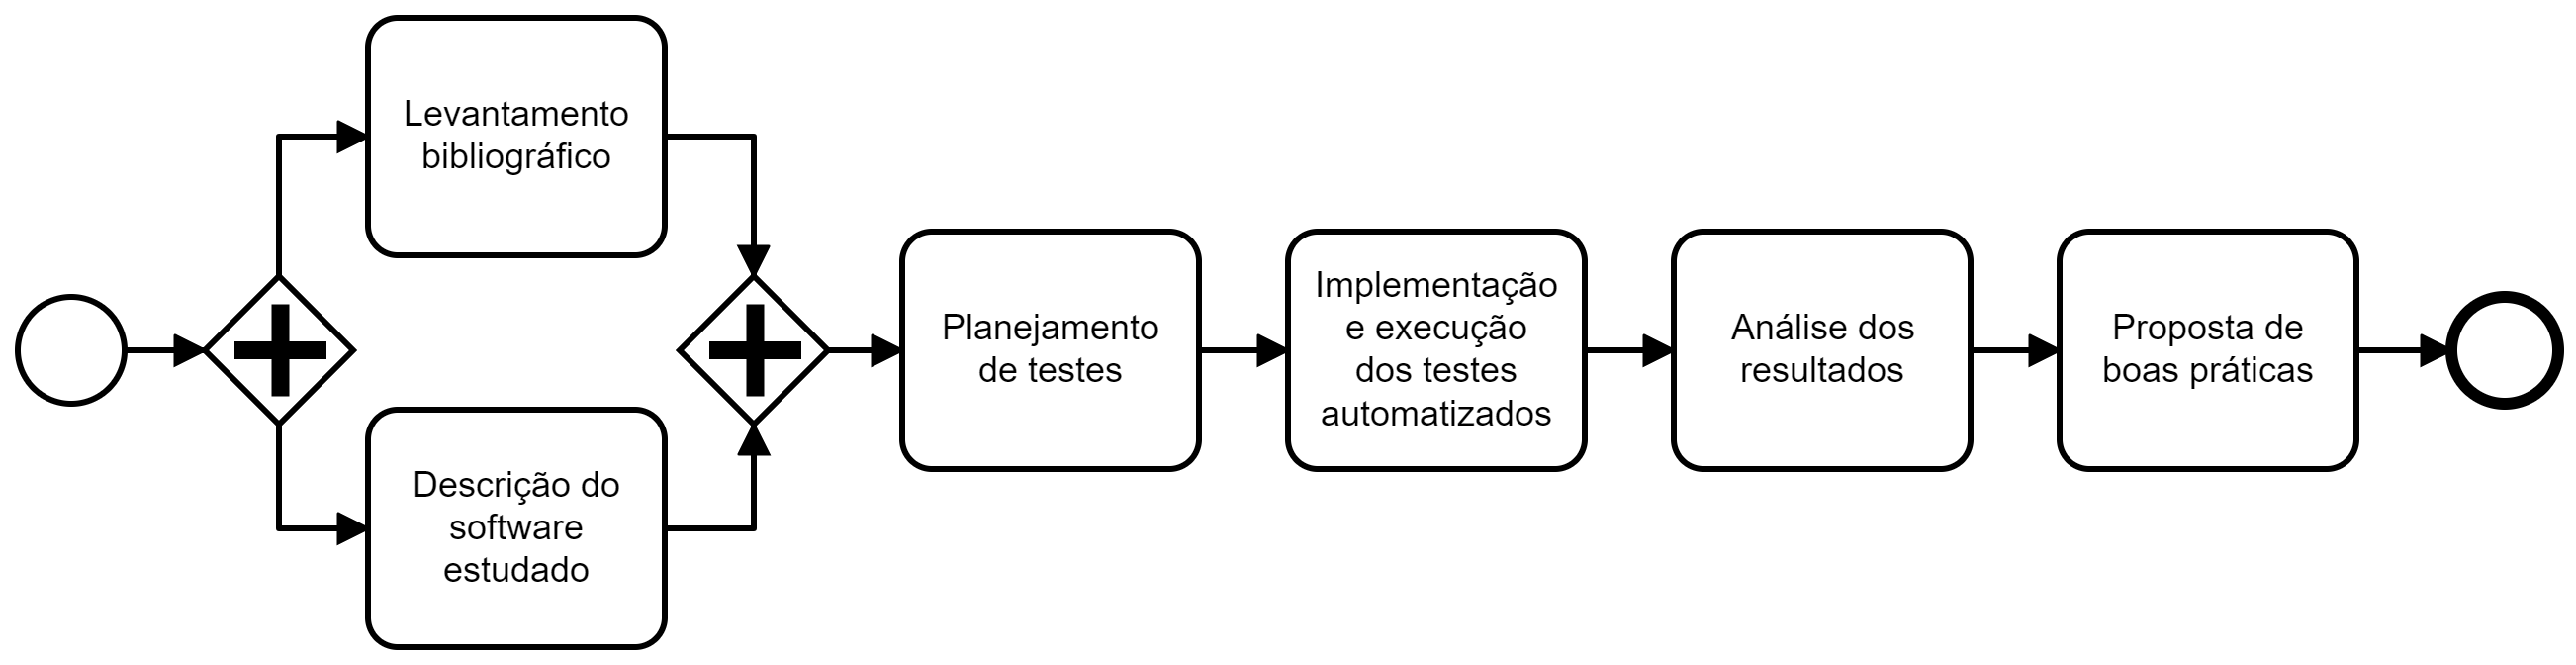
\includegraphics[width=1\textwidth]{./assets/figuras/bpmn_metodos_tcc}}% measure width
    	\begin{minipage}{\wd0}
	    	\usebox0
	    	\caption{Desenvolvimento do Trabalho}
	    	\label{fig:bpmn-metodos-tcc}
		    \fonte{o Autor}
	    \end{minipage}
    \end{figure}

   \section{DESCRIÇÃO DO SOFTWARE ESTUDADO}
    O conjunto de práticas de teste de software que pode ser aplicado em um software depende do contexto, ou seja, dependendo do processo, do projeto ou mesmo do software que é testado, algumas práticas podem ser mais apropriadas que outras. A fim de explorar a aplicação das práticas apropriadas, será realizado um estudo de caso da aplicação das práticas de teste de software nas atividades de teste do Sistema Admink.

    O Sistema Admink consiste em uma aplicação web, ou seja, um sistema de informação projetado para ser utilizado através de navegadores na internet, que foi desenvolvido há alguns meses pelo autor desta monografia e pelo estudante Thiago Teixeira durante a disciplina de Projeto do curso de Engenharia de Software da Universidade Estadual de Ponta Grossa.

    O Admink foi projetado para apoiar a administração de estúdios de tatuagem através do gerenciamento de informações importantes para o dia a dia do estúdio como dados de clientes, tatuadores, orçamentos, espaços de trabalho, agendamentos de tatuagem e indicadores de apoio à gestão. Previamente ao desenvolvimento do Sistema Admink foram produzidos documentos de casos de uso (\autoref{chap:apendiceA}) e casos de teste (\autoref{chap:apendiceB}).

    O Sistema Admink foi desenvolvido utilizando a linguagem de programação \emph{PHP} na versão 7.3.33, o \emph{framework PHP Laravel} na versão 6.20.44, e o sistema gerenciador de banco de dados relacionais de código aberto MariaDB na versão 10.4.13. O código do sistema está armazenado e versionado em um repositório no \emph{GitHub}.

    \emph{PHP} é uma linguagem de programação interpretada é direcionada para desenvolvimento para a \emph{web} com o principal objetivo de permitir a criação de páginas geradas dinamicamente rapidamente \cite{PHP2021}.

    \emph{Laravel} é um \emph{framework} para aplicações \emph{web} com sintaxe elegante e expressiva. Um \emph{framework} para aplicações \emph{web} fornece a estrutura e ponto inicial para criação das aplicações, permitindo que desenvolvedores foquem na criação da aplicação sem se preocupar com todos os detalhes. O \emph{Laravel} fornece recursos para a criação, configuração e execução de testes unitários e de integração, pois adota por padrão o \emph{PHPUnit}, que é um \emph{framework} de testes unitários para PHP \cite{Laravel2021}.

    O \emph{PHPUnit} é um um \emph{framework} de testes orientado ao programador, baseado na arquitetura \emph{xUnit} para \emph{frameworks de testes de unidade}, suportando a realização de testes automatizados. Assim como outros \emph{frameworks} de testes de unidade, o \emph{PHPUnit} utiliza asserções (\emph{assertions}) para verificar a conformidade do comportamento apresentado pelo código-fonte com o comportamento esperado. As asserções são métodos criados para garantir que o valor recebido em um teste é o valor esperado e no \emph{PHPUnit} há pelo menos 46 métodos de asserção disponíveis \cite{PHPcombr}.
    
    O Sistema Admink também conta com \emph{factories} que foram criadas durante a implementação para apoiar o desenvolvimento e a realização dos testes. As \emph{Factories} permitem que um conjunto de atributos seja definido para popular no banco de dados as tabelas de entidades que possuem classes equivalentes no código da aplicação. Quando utilizadas em conjunto com \emph{faker} o conjunto de dados pode ser gerado com valores aleatórios \cite{Laravel2021}.

    O \emph{GitHub} fornece serviços de hospedagem de repositórios baseados em nuvem, permitindo controle de versão e colaboração de forma remota.
   
    \section{LEVANTAMENTO BIBLIOGRÁFICO}

        Nesta etapa foi realizado o levantamento bibliográfico para auxílio na implementação dos testes e do entendimento do fluxo de trabalho proposto por métodos ágeis. A partir dos trabalhos encontrados descreveu-se a relação das atividades de teste de software com os processos de desenvolvimento de software e a evolução de ambos com o passar dos anos. Também foram descritas as atividades de teste de software e de testes automatizados, incluindo as técnicas utilizadas para identificação dos testes necessários para verificar aplicações de forma eficaz.

        Após entender quão amplos são os estudos de teste de software e mesmo de testes automatizados, manifestou-se a necessidade de delimitar um escopo específico como foco deste trabalho. Optou-se por estudar a implementação de testes funcionais em um dos níveis de teste automatizado para dois casos de uso do Sistema Admink. Foram escolhidos o nível de teste de integração e os casos de uso \textbf{Efetuar Login} e \textbf{Manter Orçamentos} para serem estudados neste trabalho.

    \section{PLANEJAMENTO DE TESTES}
        
        Na etapa de Planejamento de Testes foi realizada a análise de parte da documentação previamente criada do Sistema Admink, além da utilização de técnicas de teste de caixa preta para identificação dos cenários de testes. Em seguida os cenários de testes identificados foram representados em diagramas baseados em mapas mentais.

        \subsection{Representação dos cenários de teste baseada em mapas mentais}
 
            Buscando atender às necessidades de equipes que aplicam métodos ágeis com menor foco em documentações detalhadas, evitou-se a utilização de documentos extensos e que necessitem de muito tempo para serem interpretados para representação dos cenários de teste, então, propôs-se um método de representação de cenários de teste utilizando diagramas baseados em mapas mentais, contendo as principais informações necessárias para apoiar a implementação dos \emph{scripts} de testes automatizados.
            
            Mapas mentais são um método de representar informações de forma organizada e priorizada, baseado no uso de palavras-chave e imagens-chave capazes de resgatar memórias específicas, além de estimular novos pensamentos \cite{Buzan2009}.
 
            Para criação dos diagramas baseados em mapas mentais foi utilizada a aplicação web \emph{XMind}, ferramenta destinada para criação de mapas mentais e realização de \emph{brainstorm} \cite{XMind2022}. Entretanto, outras aplicações ou ferramentas voltadas para criação de diagramas baseados em mapas mentais também poderiam ser utilizadas sem prejuízos à aplicação do método. O método proposto consiste nos seguintes passos (\autoref{fig:template-mind-map-tcc}):
            
            \begin{figure}[!htb]
                \centering
	            \sbox0{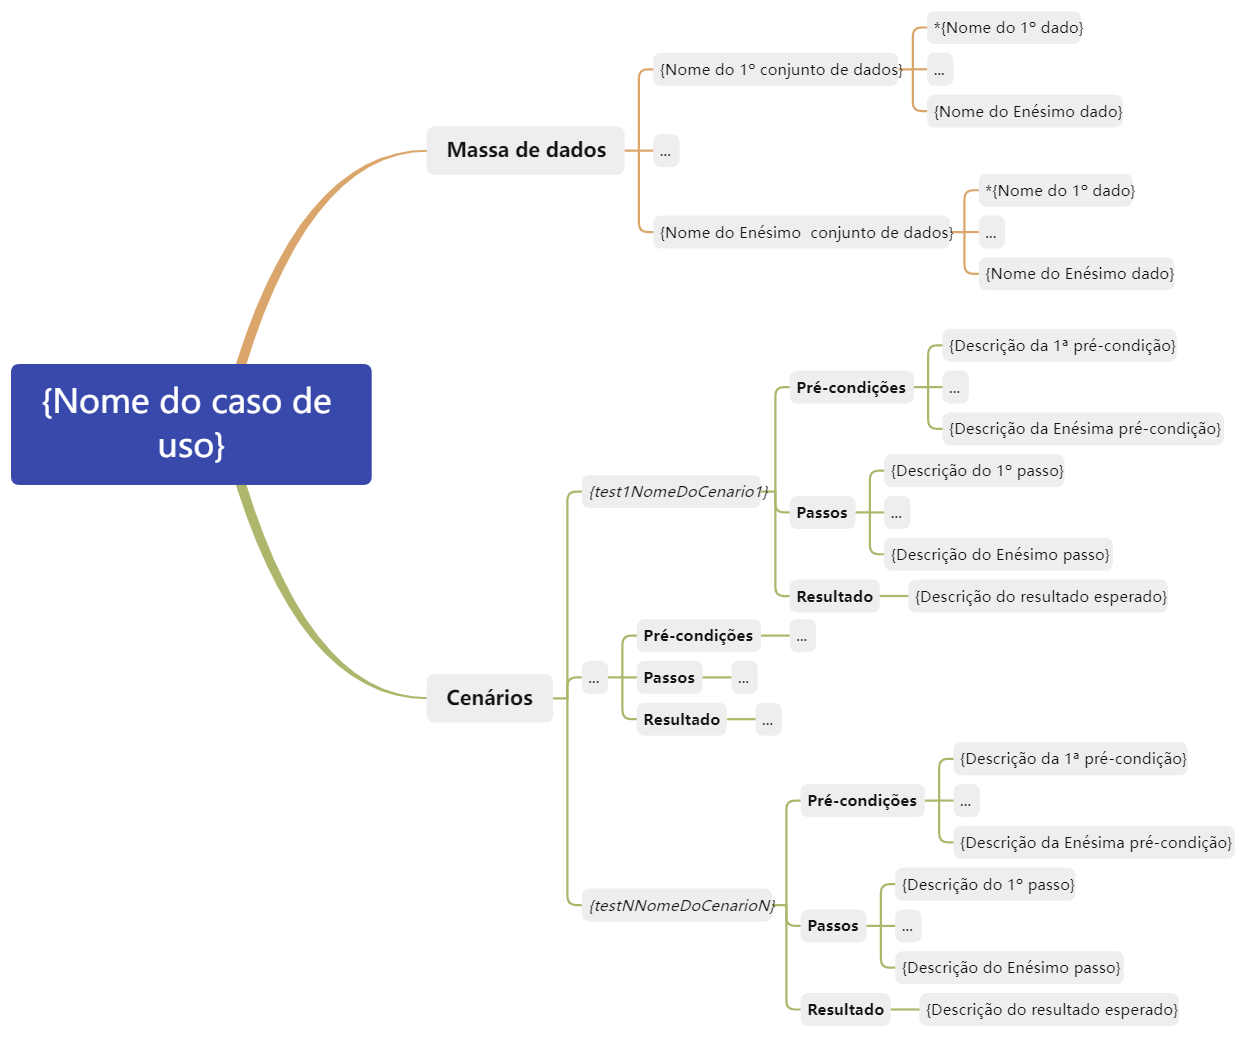
\includegraphics[width=1\textwidth]{./assets/figuras/testing_mind_map_template}}% measure width
	            \begin{minipage}{\wd0}
		            \usebox0
		            \caption{ Esquema representando o diagrama proposto pelo método para representação de cenário de testes utilizando diagramas baseados em mapas mentais onde cada um dos itens delimitados por chaves podem ser editados conforme as informações correspondente dos cenários de teste e os itens exibidos em negrito são fixos e não são editados independente das informações dos cenários de teste
		            }  
		            \label{fig:template-mind-map-tcc}
		            \fonte{o Autor}
	            \end{minipage}
            \end{figure}

            \begin{itemize}
                \item Inicia-se o digrama preenchendo a informação central do diagrama com o nome do caso de uso, história de usuário ou funcionalidade para a qual os cenários de teste serão representados;
                \item Em seguida são criados os ramos \textbf{Cenários} e \textbf{Massa de dados};
                \item A seguir são inseridos novos ramos ligados diretamente aos ramos \textbf{Cenários} e \textbf{Massa de dados}, os quais são preenchidos com as informações de cenários de testes de integração e os dados necessários para realização dos testes, respectivamente. Buscando facilitar a identificação de qual parte do código de \emph{scripts} de testes de integração corresponde a cada um dos cenários mapeados, utilizou-se a mesma nomenclatura para os ramos que representam os cenários e para o título dos métodos de teste nos \emph{scripts};
                \item Em cada um dos ramos de cenários criados são adicionados os ramos \textbf{Passos} e \textbf{Resultados}. No ramo \textbf{Passos} são descritos os passos que devem ser executados durante a realização do teste. No ramo \textbf{Resultados} é descrito o resultado que é esperado que a aplicação apresente após a execução dos passos descritos no ramo \textbf{Passos}.
            \end{itemize}
        
            Após definido o método de representação, os cenários de teste planejados para os casos de uso \textbf{Efetuar Login} e \textbf{Manter Orçamentos} foram representados utilizando o método de representação proposto. Os cenários de teste para o caso de uso \textbf{Efetuar Login} foram representandos em um único diagrama, entretanto para o caso de uso \textbf{Manter Orçamentos} foi criado um diagrama para cada funcionalidade, buscando facilitar a visualização e evitando um diagrama muito extenso.
            
    \section{IMPLEMENTAÇÃO E EXECUÇÃO DOS TESTES AUTOMATIZADOS}
        A partir da delimitação do escopo deste trabalho, consultou-se a seção \emph{Testing} da documentação da versão do \emph{Framework Laravel} utilizada no desenvolvimento do Sistema Admink a fim de descobrir as recomendações para realização de testes de integração. Descobriu-se que projetos criados a partir do \emph{Framework Laravel} já são pré-configurados por padrão com os recursos para criação de testes unitários e de integração, utilizando \emph{PHPUnit}, e que é recomendado utilizar esses recursos para a criação dos \emph{scripts} de testes automatizados.
 
        Após os cenários de testes estarem representados nos diagramas baseados em mapas mentais, iniciou-se a codificação dos \emph{scripts} de testes de integração automatizados utilizando os diagramas como base e seguindo as instruções da documentação do \emph{Framework Laravel} e do \emph{PHPUnit}. Além dos diagramas, o código foi analisado para entender como a aplicação está estruturada e quais partes do código deveriam ser utilizadas para realização dos testes.
        
        Baseando-se nas informações fornecidas pelos diagramas cada um dos \emph{scripts} de teste foi criado utilizando o framework para testes de unidade emph{PHPUnit} na versão 9.5.17. Cada um dos itens de cada diagrama foi analisado para criar os \emph{scripts} de teste:
        
        \begin{itemize}
            \item Inicialmente foi criada uma classe por digrama para conter os métodos referentes aos cenários de teste representados em cada diagrama;
            \item Em seguida analisou-se as informações presentes nos itens referentes a \textbf{Massa de dados} para identificar os dados necessários para realização dos testes e como prepará-los para serem utilizados nos \emph{scripts};
            \item A partir dos itens referentes aos \textbf{Cenários} são criados métodos de teste com os mesmos nomes mostrados nos diagramas;
            \item A partir dos itens referentes às \textbf{Pré-condições} são implementados nos métodos de teste as ações que devem ser realizadas antes dos passos de cada teste;
            \item A partir dos itens referentes aos \textbf{Passos} são implementadas nos métodos as ações que que devem causar os resultados esperados na aplicação;
            \item Por fim, as asserções são criadas nos métodos de teste esperando como retorno da aplicação as mesmas informações presentes nos itens referentes ao \textbf{Resultado} de cada cenário de teste presente no diagrama.
        \end{itemize}
        
        Após criados os \emph{scripts} de teste foi realizada a execução dos mesmos em um computador equipado com o Sistema Operacional Windows 10 Pro na versão 21H1, com processador Intel(R) Core(TM) i5-10210U de 1.60GHz, com 16 GB de memória principal e com uma unidade de estado sólido de 256 GB. Foram realizados 30 execuções sucessivas dos \emph{scripts} de teste criados e coletados os dados de tempo de execução para calcular-se o tempo médio gasto nessas execuções.
        
        Os resultados obtidos após a realização dos métodos e experimentos acima descritos serão explorados no \autoref{chap:resultados}.                    % Metodologia
% RESULTADOS-------------------------------------------------------------------

\chapter{RESULTADOS E DISCUSSÕES}
\label{chap:resultados}

Utilizando o método de representação de cenários de teste utilizando diagramas baseados em mapas mentais foram criados diagramas para representar cada um dos cenários de teste automatizados para as funcionalidades \textbf{Efetuar Login} (\autoref{fig:testing-mind-map-efetuar-login}), \textbf{Cadastro de Orçamentos} (\autoref{fig:testing-mind-map-orcamentos-cadastro}), \textbf{Listagem e Deleção de Orçamentos} (\autoref{fig:testing-mind-map-orcamentos-listagem-e-delecao}) e \textbf{Edição de Orçamentos} (\autoref{fig:testing-mind-map-orcamentos-edicao}).

            \begin{figure}[!htb]
                \centering
	            \sbox0{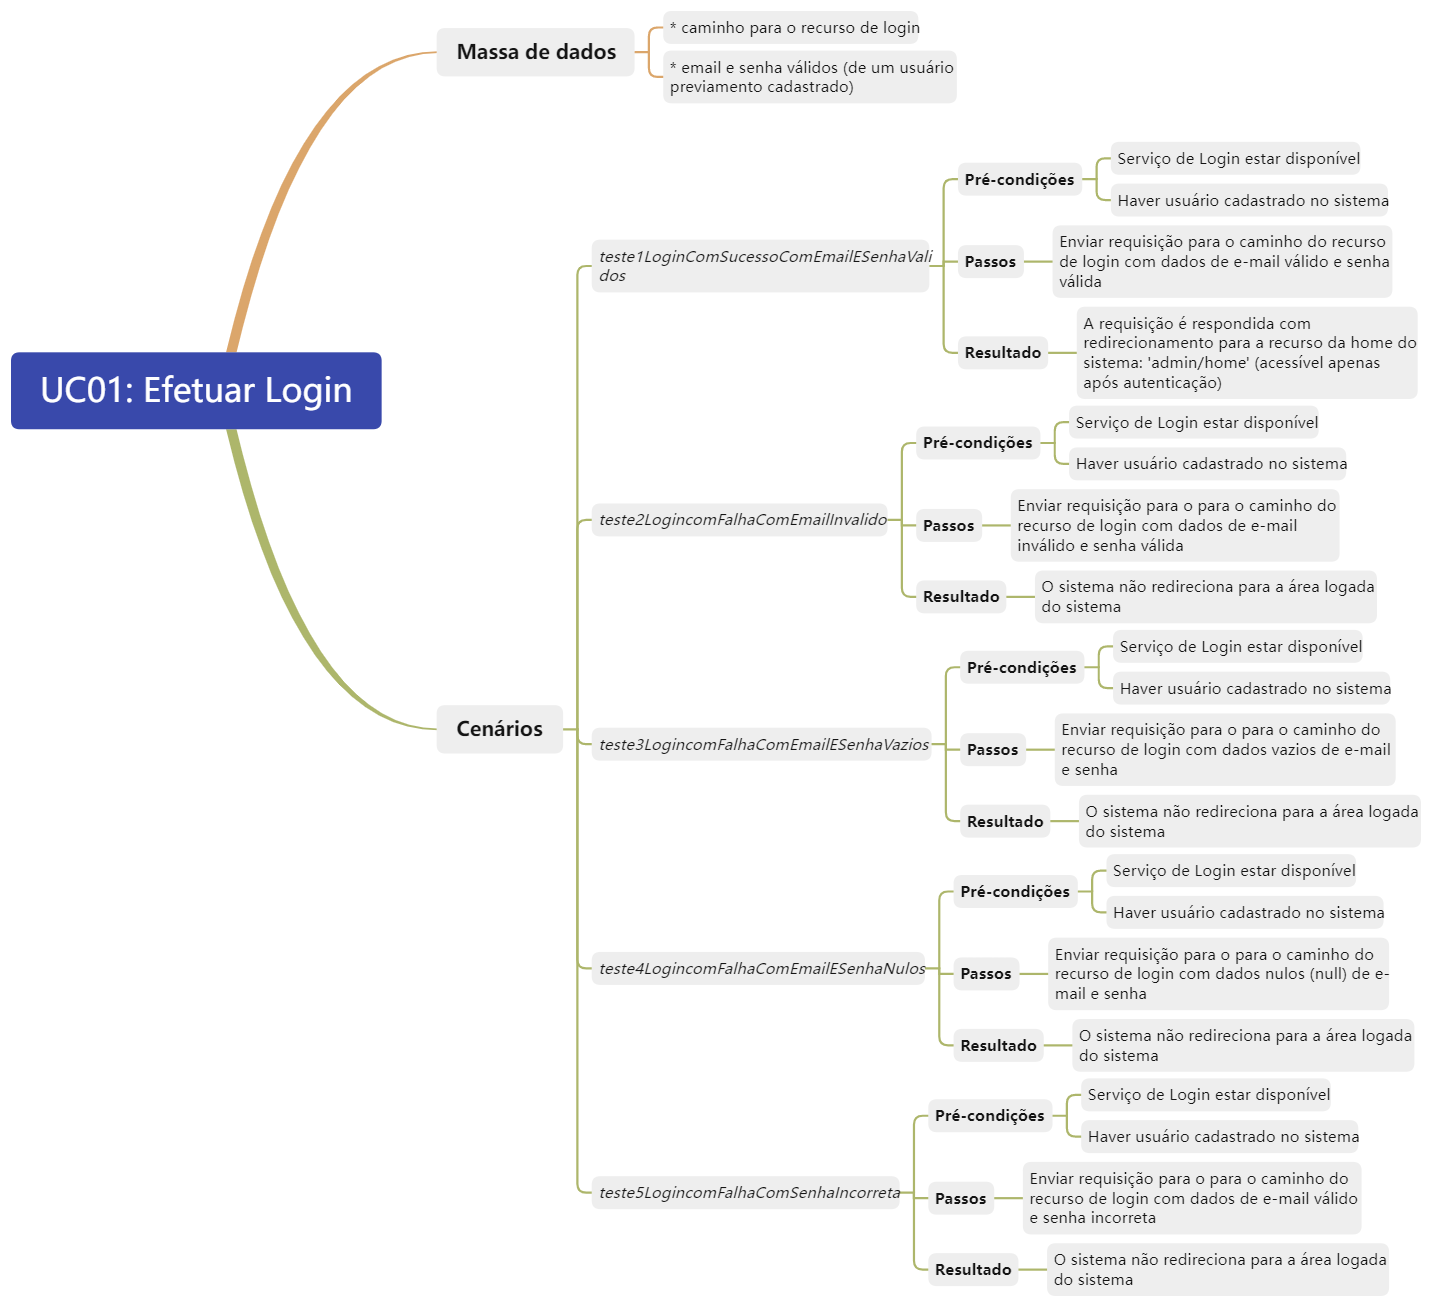
\includegraphics[width=1\textwidth]{./assets/figuras/testing-mind-map-efetuar-login}}% measure width
	            \begin{minipage}{\wd0}
		            \usebox0
		            \caption{Diagrama representando os cenários de teste da funcionalidade \textbf{Efetuar Login}} % Implementação dos cenários de teste de login, baseado na documentação do software e 
		            \label{fig:testing-mind-map-efetuar-login}
		            \fonte{o Autor}
	            \end{minipage}
            \end{figure}

            \begin{figure}[!htb]
                \centering
	            \sbox0{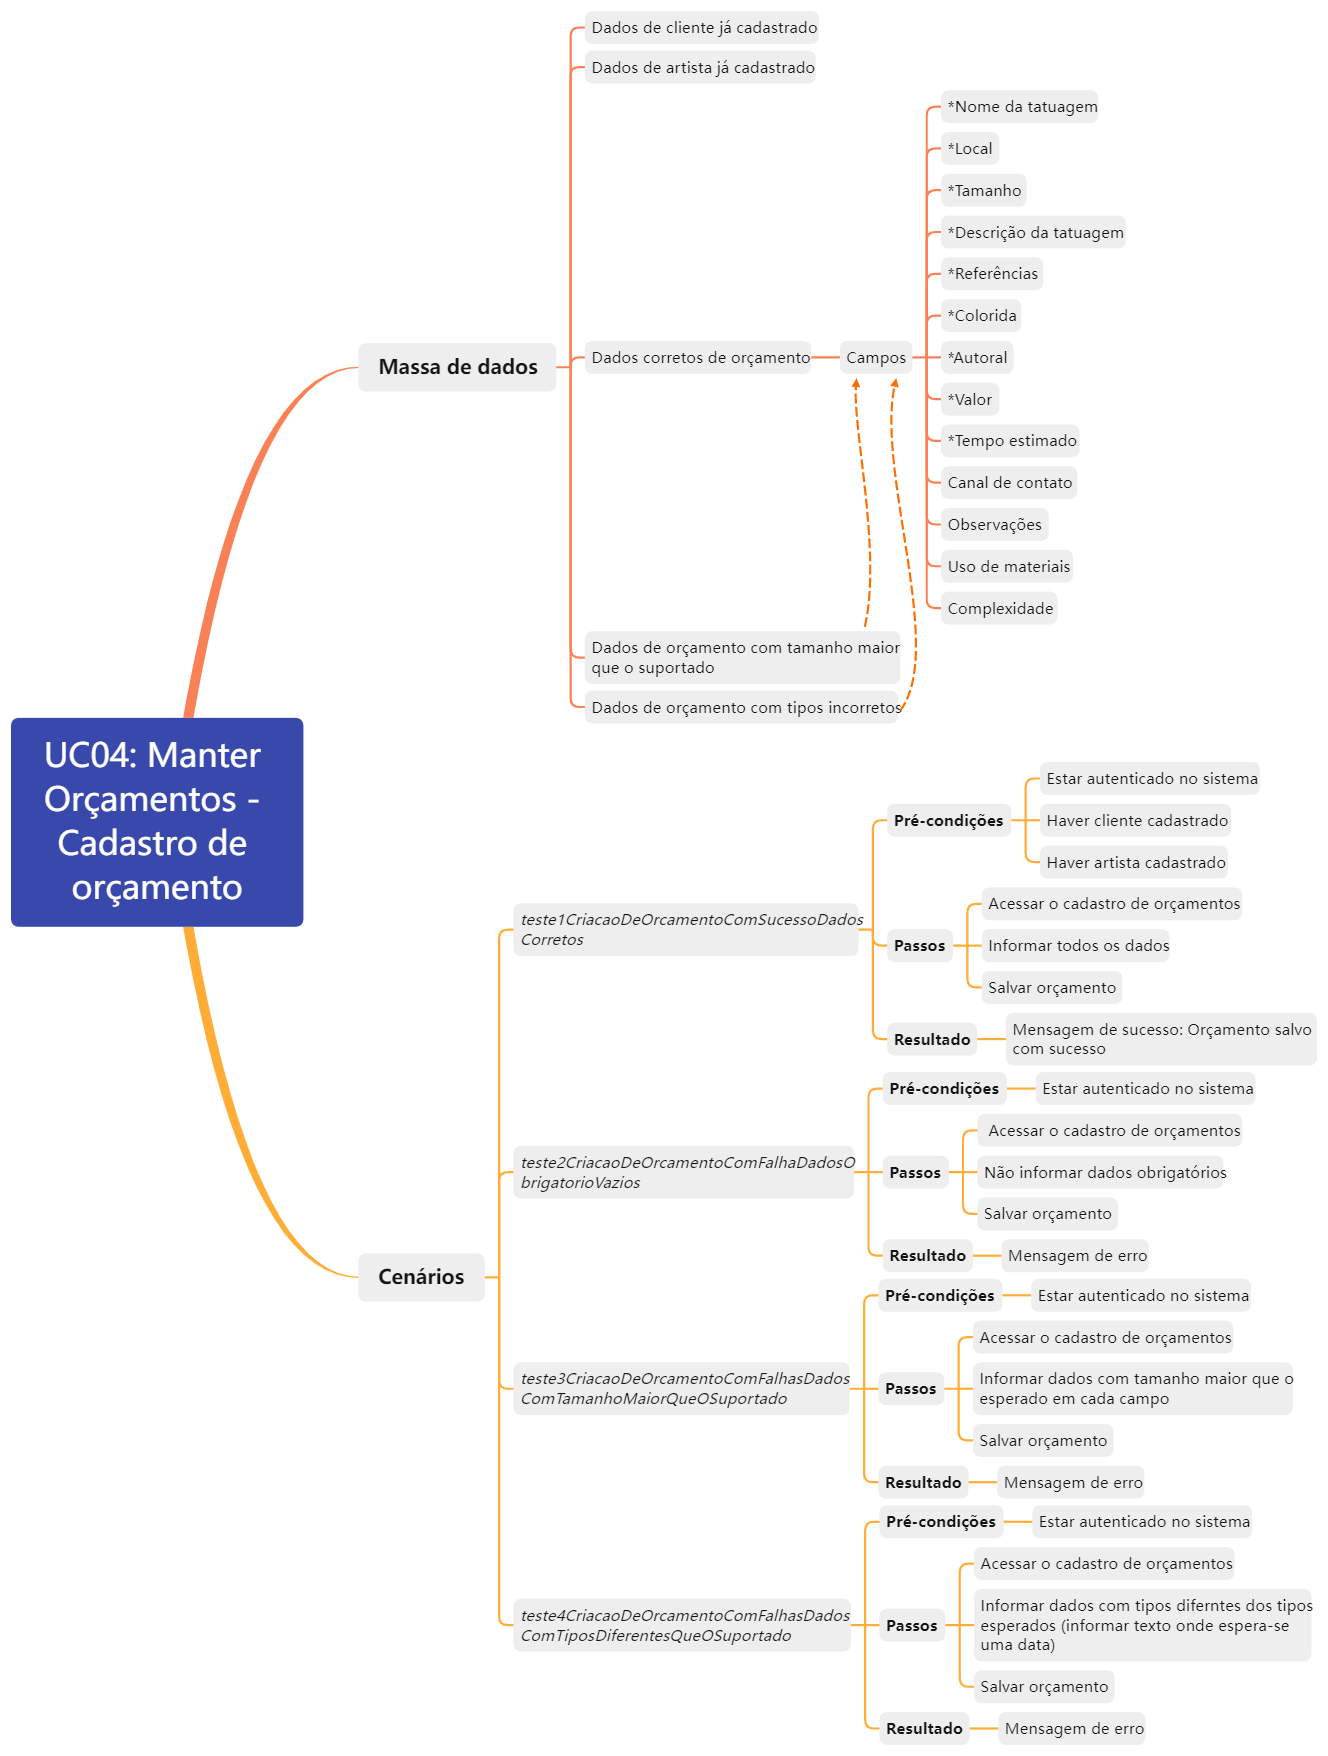
\includegraphics[width=1\textwidth]{./assets/figuras/testing-mind-map-orcamentos-cadastro}}% measure width
	            \begin{minipage}{\wd0}
		            \usebox0
		            \caption{Diagrama representando os cenários de teste da funcionalidade \textbf{Cadastro de Orçamentos}}
		            \label{fig:testing-mind-map-orcamentos-cadastro}
		            \fonte{o Autor}
	            \end{minipage}
            \end{figure}

            \begin{figure}[!htb]
                \centering
	            \sbox0{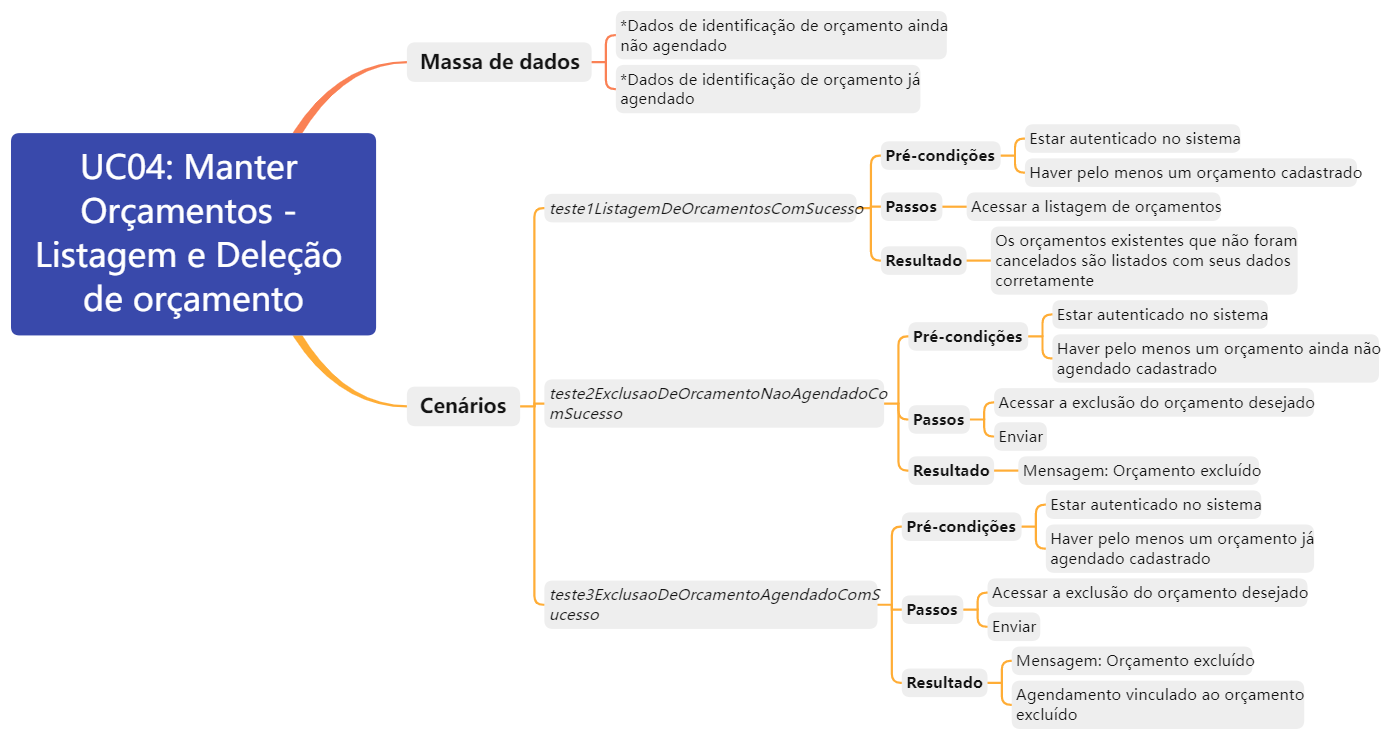
\includegraphics[width=1\textwidth]{./assets/figuras/testing-mind-map-orcamentos-listagem-e-delecao}}% measure width
	            \begin{minipage}{\wd0}
		            \usebox0
		            \caption{Diagrama representando os cenários de teste das funcionalidades \textbf{Listagem e Deleção de Orçamentos}}
		            \label{fig:testing-mind-map-orcamentos-listagem-e-delecao}
		            \fonte{o Autor}
	            \end{minipage}
            \end{figure}

            \begin{figure}[!htb]
                \centering
	            \sbox0{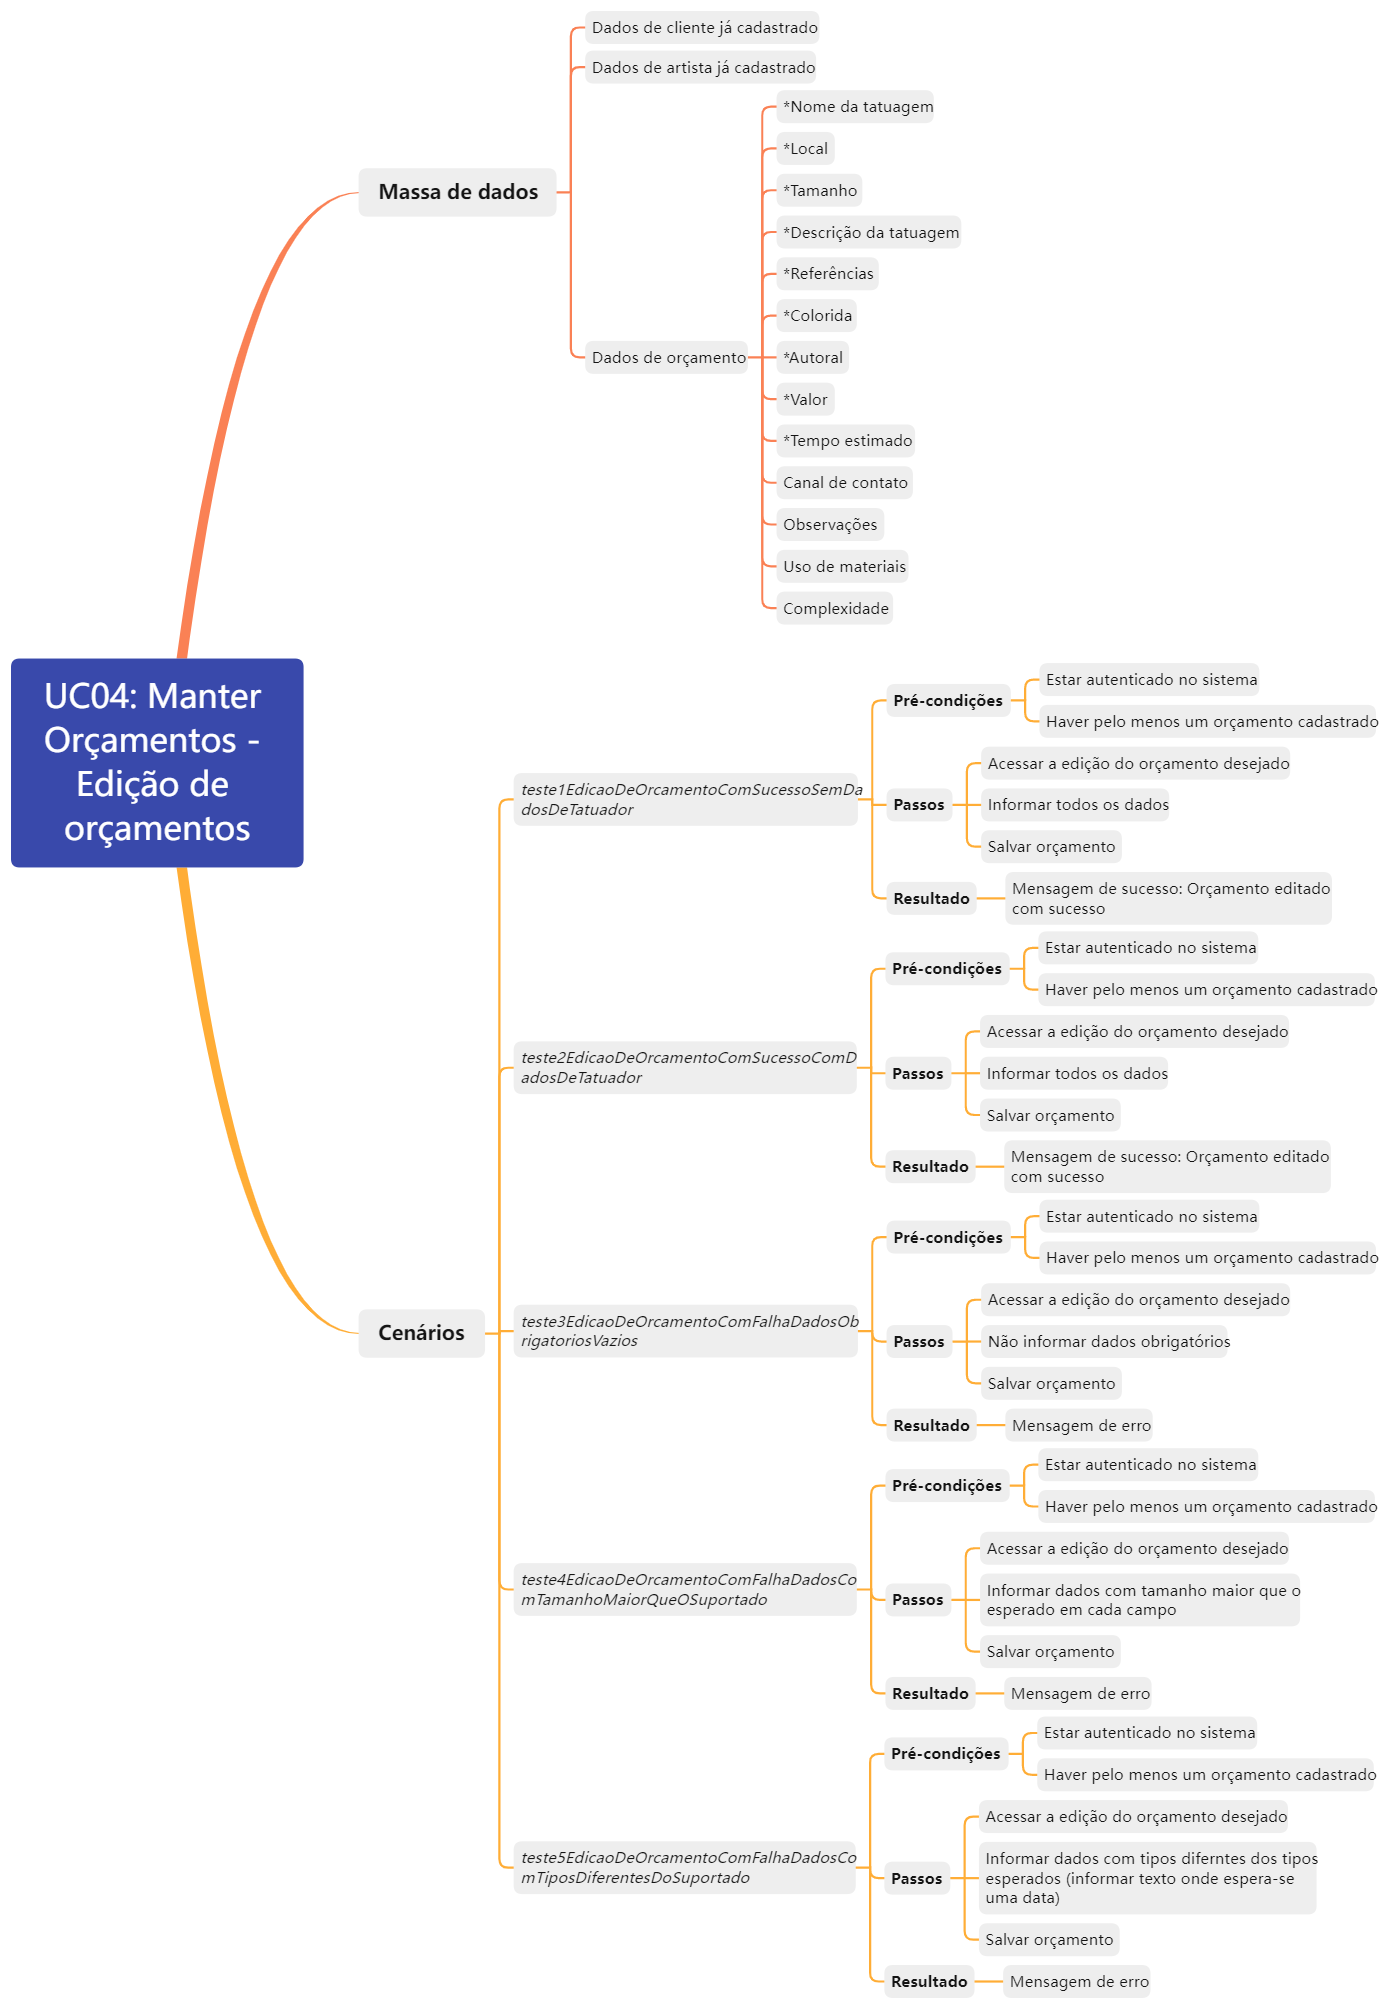
\includegraphics[width=1\textwidth]{./assets/figuras/testing-mind-map-orcamentos-edicao}}% measure width
	            \begin{minipage}{\wd0}
		            \usebox0
            		\caption{Diagrama representando os cenários de teste das funcionalidades \textbf{Edição de Orçamentos}}
		            \label{fig:testing-mind-map-orcamentos-edicao}
		            \fonte{o Autor}
	            \end{minipage}
            \end{figure}

    Em seguida foram criados os \emph{scripts} de teste de integração para os cenários de teste mapeados. O primeiro \emph{script} criado, contém os testes do caso de uso \textbf{Efetuar Login} (\autoref{code:logintest}):
        
    \begin{itemize}
        \item O \emph{script} de teste começa com a declaração da classe de teste e as importações utilizadas nos \emph{scripts} de testes (linhas 1 a 9);
        \item Os métodos de teste são declarados, com o título iniciando sempre pela palavra teste, seguindo a mesma nomenclatura dada aos cenários nos diagramas de planejamento de testes (linha 11);
        \item Abaixo da declaração do método de teste, os objetos e variáveis utilizados no testes são declaradas e instanciadas para serem utilizados nas chamadas (linha 13);
        \item É feita a requisição para o recurso correspondente à funcionalidade testada com os dados de envio necessários, conforme a aplicação foi desenvolvida. A resposta da requisição é armazenada na variável \emph{response} (linha 14);
        \item A asserção verifica o \emph{status code} do retorno da requisição (linha 15) e o redirecionamento para a área do Sistema Admink que é acessível apenas após estar autenticado (linha 16).
    \end{itemize}
        
    %Python code highlighting
\begin{lstlisting}[language=PHP, caption= Cenários de Testes Automatizados de Integração do Login,label={code:logintest}]
<?php

namespace Tests\Integration\Login;

use Tests\TestCase;
use App\User;

class LoginTest extends TestCase
{

    public function teste1LoginComSucessoComEmailESenhaValidos()
    {
        $user = factory(User::class)->create();
        $response = $this->call('POST', '/login', ['email' => $user->email, 'password' => 'teste@123']);
        $response->assertStatus(302);
        $response->assertRedirect('/admin/home');
    }
    
\end{lstlisting}

\fonte{o Autor}
        
    O código realiza a requisição enviando os dados presentes no \emph{script} de teste e por meio das asserções verifica o que foi retornado pelo sistema. Caso o retorno dado pelo sistema seja o esperado na asserção, o teste obtém sucesso, caso contrário o teste falha.
        
    Os objetos instanciados a partir de classes do Sistema Admink foram criados dentro dos \emph{scripts} de teste através das \emph{factories} criadas durante o desenvolvimento do Sistema Admink. As \emph{factories} permitem que os objetos sejam criados com dados aleatórios, possibilitando que diferentes execuções dos testes utilizem diferentes dados, além de permitirem que os comandos para criação dos dados estejam dentro do \emph{script} de teste, removendo a necessidade de que outros \emph{scripts} ou instruções sejam executadas antes dos testes. O uso de \emph{factories} também possibilitou a utilização de um banco de dados \emph{SQLite} específico para os testes. % incluir exemplo no apêndice
        
    Comparando o \emph{script} de teste do cenário  \emph{teste1LoginComSucessoComEmailESenhaValidos} com o diagrama de planejamento de testes é possível visualizar qual parte do \emph{script} cada ramo representa (\autoref{fig:code-and-mind-map}).
        
    \begin{figure}[!htb]
        \centering
	    \sbox0{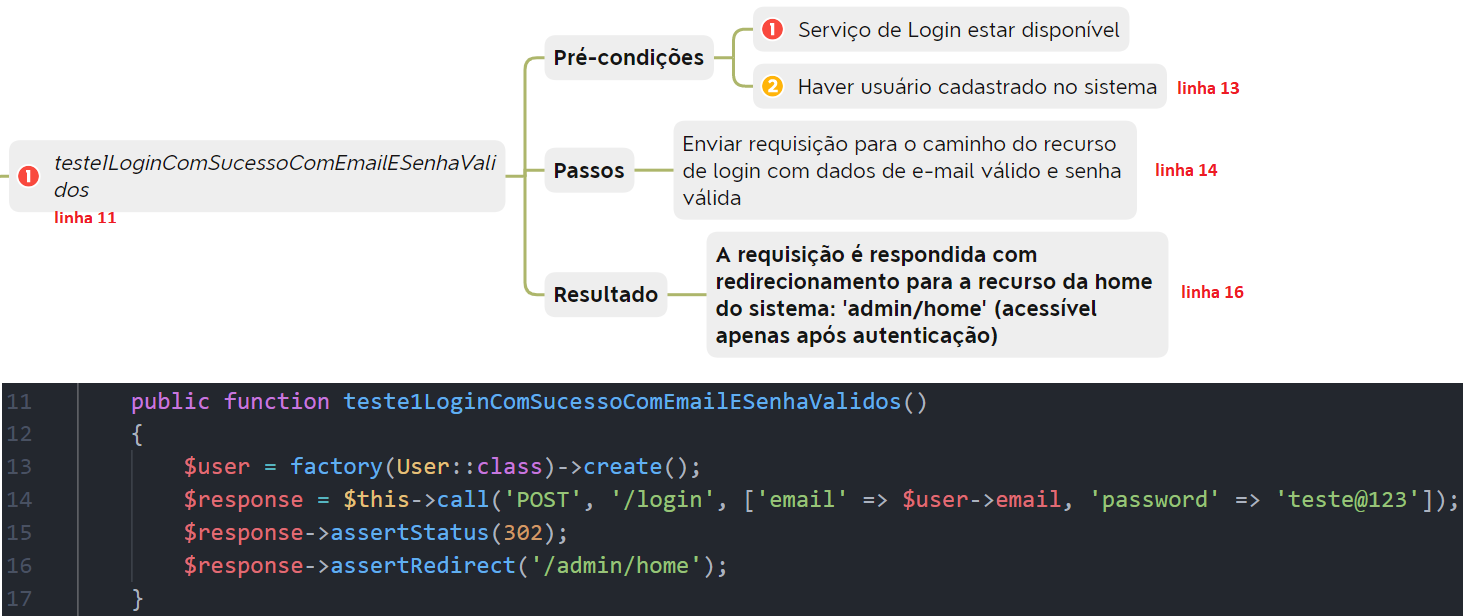
\includegraphics[width=1\textwidth]{./assets/figuras/code-and-mind-map}}% measure width
        \begin{minipage}{\wd0}
	        \usebox0
	        \caption{Comparação do diagrama com o script de teste}
	        \label{fig:code-and-mind-map}
	        \fonte{o Autor}
        \end{minipage}
    \end{figure}
        
    Para cada cenário do caso de uso \textbf{Efetuar Login} deve ser elaborado os \emph{scripts} de teste seguindo uma estrutura semelhante ao primeiro cenário descrito, com as respectivas instâncias de dados e asserções que representam o cenário e sua regra de negócio, pois alterando-se os dados de entrada alteraram-se também o comportamento e os resultados esperados.
        
    Os \emph{scripts} de teste para os cenários de teste identificados para as funcionalidades do caso de uso \textbf{Manter Orçamentos} foram criados seguindo uma estrutura similar à dos testes do caso de uso \textbf{Efetuar Login}. O código completo com todos os \emph{scripts} de teste criados pode ser encontrado no (\autoref{chap:apendiceC}).
    % referenciar apêndices
 
    Utilizando a estrutura definida pelo framework \emph{Laravel}, foi realizada a configuração necessária para a execução dos \emph{scripts} de teste nos arquivos de configuração do \emph{PHPunit} e de variáveis de ambiente.
        
    Em seguida os testes criados foram executados e os resultados analisados.
        
    Todos os \emph{scripts} criados foram armazenados no repositório privado do projeto Admink no \emph{Github}, mas também foi criado um repositório público para armazenar e compartilhar o que foi desenvolvido neste trabalho \footnote{https://github.com/QAkarotto/tcc-software-2022}.
        
    Após os testes criados terem sido executados, analisaram-se os resultados das execuções através dos relatório de execução fornecidos pelo \emph{PHPunit} após o término de cada execução (\autoref{fig:test-result}). Foram realizadas 30 execuções sucessivas, e em todas elas os 19 testes e 84 asserções criadas nos \emph{scripts} de teste obtiveram sucesso em suas execuções, não apresentando falhas. O tempo de execução em todas as execuções não ultrapassou 3 segundos e em média levou cerca de 1,6132 segundos (\autoref{tab:execucaoDosTestes}).
    
    \begin{figure}[!htb]
        \centering
        \sbox0{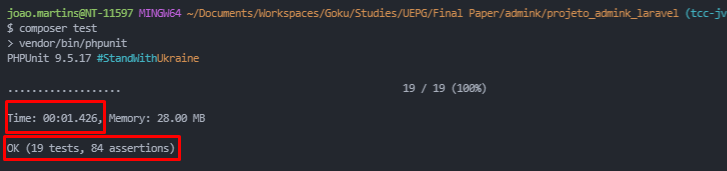
\includegraphics[width=1\textwidth]{./assets/figuras/test-result}}% measure width
        \begin{minipage}{\wd0}
	        \usebox0
	        \caption{Relatório da execução dos testes automatizados destacando em vermelho o tempo de execução e a quantidade de testes e asserções realizadas com sucesso}
	        \label{fig:test-result}
	        \fonte{o Autor}
        \end{minipage}
    \end{figure}
    
    \begin{table}[!htb]
    \vspace{0.5cm}
    \centering
    \begin{tabularx}{\textwidth}{rrrrr}
        \toprule
    & Nº da Execução & Tempo de execução (segundos) \\
        \midrule
             1ª execução	&	1.426	\\
             2ª execução	&	1.312	\\
             3ª execução	&	1.331	\\
             4ª execução	&	1.35	\\
             5ª execução	&	1.383	\\
             6ª execução	&	1.347	\\
             7ª execução	&	1.402	\\
             8ª execução	&	1.365	\\
             9ª execução	&	1.342	\\
            10ª execução &	1.348	\\
            11ª execução &	1.313	\\
            12ª execução &	1.409	\\
            13ª execução &	1.337	\\
            14ª execução &	1.364	\\
            15ª execução &	1.443	\\
            16ª execução &	1.449	\\
            17ª execução &	1.384	\\
            18ª execução &	1.322	\\
            19ª execução &	2.359	\\
            20ª execução &	2.516	\\
            21ª execução &	2.171	\\
            22ª execução &	1.814	\\
            23ª execução &	1.955	\\
            24ª execução &	1.968	\\
            25ª execução &	1.861	\\
            26ª execução &	1.816	\\
            27ª execução &	1.837	\\
            28ª execução &	1.989	\\
            29ª execução &	1.86	\\
            30ª execução &	1.624	\\
        \bottomrule
         Média & 1.613233333
    \end{tabularx}
	\caption[Resultados das execuções scripts de testes]{Resultados das execuções \emph{scripts} de testes.\label{tab:execucaoDosTestes}}
    \fonte{o Autor.}
\end{table}

    
    Foram inseridas alterações nos dados de envio de um dos testes para verificar o que é retornado no relatório de execução em caso de testes falharem. No relatório são exibidas informações indicando quantas falhas foram encontradas, em qual arquivo estão as asserções que falharam, quais asserções falharam e quais foram os valores obtidos comparados aos valores esperados nas asserções, evidenciando o motivo do teste falhar (\autoref{fig:test-fail}).
    
    \begin{figure}[!htb]
        \centering
        \sbox0{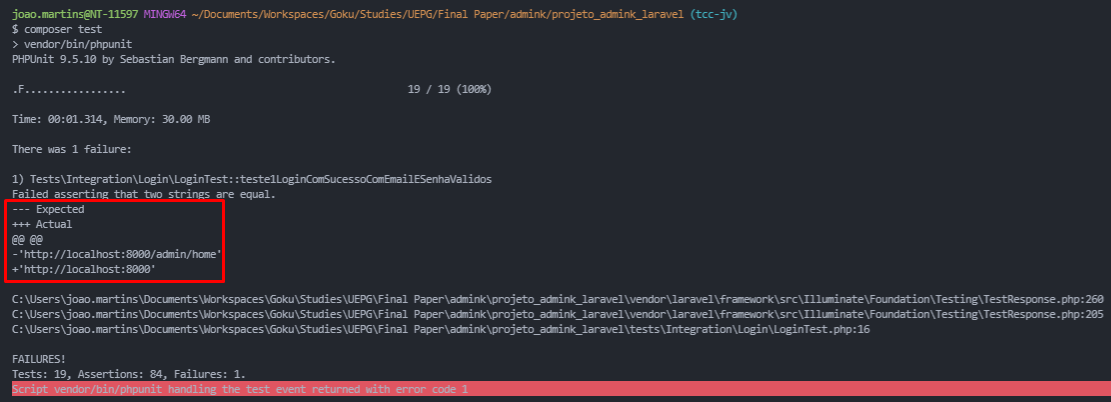
\includegraphics[width=1\textwidth]{./assets/figuras/test-fail-tcc}}% measure width
        \begin{minipage}{\wd0}
	        \usebox0
	        \caption{Exemplo de um teste cuja asserção falhou}
	        \label{fig:test-fail}
	        \fonte{o Autor}
	    \end{minipage}
    \end{figure}
        
    Com os \emph{scripts} criados e suas execuções obtendo sucesso para todos os testes e asserções em poucos segundos, entende-se que a metodologia aplicada na implementação dos testes de integração automatizados foi bem-sucedida e as práticas utilizadas podem ser consideradas para a implementação de testes automatizados de integração. 
    
    Como recomendações propostas por este trabalho, para desempenhar atividades de teste de maneira eficiente deve-se:
    
    \begin{itemize}
        \item Realizar o planejamento dos testes, baseando-se na especificação dos requisitos do software e na aplicação de técnicas de caixa preta, visando identificar os cenários de teste que serão automatizados e quais são os conjuntos de dados que devem ser utilizados nos testes. Caso os \emph{scripts} de teste sejam definidos após a criação do código fonte do software testado, o próprio código fonte somado à aplicação de técnicas de caixa branca pode ser utilizado para auxiliar na identificação dos cenários de teste. Recomenda-se também o uso do método para construção de diagramas de planejamento de testes baseados em mapas mentais como forma de representação dos cenários de teste, evitando a criação de documentos extensos e detalhados;
        \item Consultar a documentação da linguagem de programação ou \emph{framework} utilizado no desenvolvimento do software que será testado, e seguir as recomendações dadas pela documentação a respeito dos \emph{scripts} de teste e configurações necessárias para criação e execução dos mesmos;
        \item Nomear os métodos de teste de acordo com as recomendações da documentação da ferramenta, além de usar a mesma nomenclatura utilizada nos nomes dos cenários de teste identificados. Os nomes devem transmitir claramente o que está sendo verificado pelo método de teste. Desta forma, apesar da nomenclatura dos métodos se tornar verbosa, ela fornece sentido semântico mais rico, e possibilita que os próprios \emph{scritps} de teste sejam parte da documentação do software;
        \item Evitar criar dependências entre diferentes métodos de teste, possibilitando que os métodos possam ser executados em qualquer ordem sem que os testes falhem. Ou seja, os dados e pré-condições necessárias para a execução de um método de teste devem ser providos pelo próprio método, ou então, por um método auxiliar de configuração que é executado antes de todo método de teste ser executado;
        \item Utilizar bancos de dados criados especificamente para os testes, evitando que possua dados que não foram inseridos pelos testes ou como preparação para a execução dos testes. Com o apoio de \emph{migrations} \footnote{permite que o esquema (\emph{schema}) do banco de dados seja definido e possa ser compartilhado,bastando executar a \emph{migration} para atualizar o esquema, além de serem agnósticas de banco de dados, possibilitando a utilização do mesmo código de \emph{migrations} em qualquer sistema gerenciador de banco de dados utilizado} e \emph{factories}, um banco de dados pode ser facilmente criado e populado a cada execução dos testes. Caso não seja possível criar um banco de dados específico para execução dos testes, podem ser utilizados \emph{mock objects}. Entretanto, dessa última forma, não haverá comunicação com um banco de dados real;
        \item Utilizar asserções que obtenham sucesso apenas quando o comportamento esperado realmente foi apresentado pela aplicação. Ou seja, as asserções devem ser precisas e devem evidenciar que o resultado esperado foi obtido.
        \item Armazenar o código criado em um repositório;
    \end{itemize}
    
    As recomendações propostas colaboram para que os \emph{scripts} de teste atendam aos princípios \emph{FISRT} e não possuam \emph{test smells} (\autoref{chap:teste-de-software}) e podem ser inseridas no fluxo de times que utilizam o XP como método ágil, podendo ser realizadas durante a prática do Desenvolvimento Guiado por Testes. Mas também podem ser utilizadas por outros times que também desejem implementar testes automatizados sem ter que criar documentos extensos e detalhados.
    
    Durante a implementação dos testes algumas dificuldades foram encontradas para realizar as asserções devido a forma que a aplicação foi desenvolvida. Nas respostas das requisições realizadas pelos \emph{scripts} de teste sempre é retornado um documento \emph{HTML} como resposta. Dessa forma as asserções devem ser realizadas comparando o conteúdo de campos do \emph{HTML} retornado com os valores esperados. Foi necessário analisar o \emph{HTML} retornado para identificar quais campos continham os dados esperados. Por exemplo no \emph{script} do teste \textbf{teste1ListagemDeOrcamentosComSucesso}  (\autoref{code:teste1ListagemDeOrcamentosComSucesso}):
    
    \begin{itemize}
        \item Nas linhas 18 a 22 é possível visualizar que as asserções estão verificando se o documento \emph{HTML} contem os elementos esperados.
    \end{itemize}
    
    \begin{lstlisting}[language=PHP, caption= Script do teste teste1ListagemDeOrcamentosComSucesso,label={code:teste1ListagemDeOrcamentosComSucesso}]

public function teste1ListagemDeOrcamentosComSucesso()
    {
        $user = factory(User::class)->create();
        $estudio = factory(Estudio::class)->create();
        factory(EstudioUsers::class)->create(['fk_users_id_users' => $user->id, 'fk_estudio_id_estudio' => $estudio->id_estudio]);
        $artista = factory(Artista::class)->create();
        $cliente = factory(Cliente::class)->create();
        factory(ArtistaEstudio::class)->create(['fk_artista_id_artista' => $artista->id_artista, 'fk_estudio_id_estudio' => $estudio->id_estudio]);
        factory(ClienteEstudio::class)->create(['fk_cliente_id_cliente' => $cliente->id_cliente, 'fk_estudio_id_estudio' => $estudio->id_estudio]);
        $orcamento = factory(Orcamento::class)->create(['fk_cliente_id_cliente' => $cliente->id_cliente, 'fk_artista_id_artista' => $artista->id_artista, 'fk_estudio_id_estudio' => $estudio->id_estudio, 'fk_orcamento_status_id_orcamento_status' => 1]);
        $orcamento2 = factory(Orcamento::class)->create(['fk_cliente_id_cliente' => $cliente->id_cliente, 'fk_artista_id_artista' => $artista->id_artista, 'fk_estudio_id_estudio' => $estudio->id_estudio, 'fk_orcamento_status_id_orcamento_status' => 1]);

        $response = $this->actingAs($user)
            ->get('/admin/orcamentos');

        $response->assertStatus(200);
        $response->assertSee('<td class="align-middle">' . $orcamento->tatuagem_nome . '</td>', $escaped = false);
        $response->assertSee('<td class="align-middle">#' . str_pad($orcamento->id_orcamento, 5, '0', STR_PAD_LEFT) . '</td>', $escaped = false);
        $response->assertSee('<td class="align-middle">' . $orcamento2->tatuagem_nome . '</td>', $escaped = false);
        $response->assertSee('<td class="align-middle">#' . str_pad($orcamento2->id_orcamento, 5, '0', STR_PAD_LEFT) . '</td>', $escaped = false);
    }
    
\end{lstlisting}

\fonte{o Autor}
    
    Caso o Sistema Admink tivesse sido desenvolvido para responder as requisições retornando os dados em um documento \emph{JSON} ao invés de diretamente no \emph{HTML} da interface gráfica, a identificação dos campos contendo os dados esperados seria facilitada, assim como a criação das asserções, pois seria necessário verificar apenas os dados do \emph{JSON} e não todo o \emph{HTML}. nas linhas 8 a 10 do \emph{script} de exemplo extraído da documentação do \emph{Framework Laravel} é possível ver como são realizadas asserções para campos de documentos \emph{JSON} (\autoref{code:JSONExampleTest}).
   
    %Python code highlighting
\begin{lstlisting}[language=PHP, caption= Script de Teste exemplificando asserções baseadas em campos de documentos \emph{JSON},label={code:JSONExampleTest}]

public function test_making_an_api_request()
    {
        $response = $this->postJson('/api/user', ['name' => 'Sally']);
 
        $response
            ->assertStatus(201)
            ->assertJson([
                'created' => true,
            ]);
    }
    
\end{lstlisting}

\fonte{o Autor}
    
    Também foram encontradas dificuldades com asserções utilizando os \emph {status codes} retornados nas respostas das requisições. A maioria das requisições realizadas para o Sistema Admink retornam o mesmo \emph{status code} tanto quando se obtém sucesso como quando falha. Para diferenciar sucessos de erros foi necessário analisar as mensagens de sucesso e de erro retornadas nas respostas das requisições, além de utilizar tais mensagens na criação das asserções. Por exemplo nos \emph{scripts} \textbf{teste1CriacaoDeOrcamentoComSucessoDadosCorretos} e \textbf{teste2CriacaoDeOrcamentoComFalhaDadosObrigatorioVazios} (\autoref{code:CriacaoDeOrcamentoTest1E2}):
    
            \begin{itemize}
        \item Na linha 30 é possível ver que a asserção está sendo realizada para o \emph{status code} 302;
        \item Na linha 31 é realizada uma asserção para o texto da mensagem de sucesso na criação de orçamento;
        \item Na linha 58 é realizada asserção também para o \emph{status code} 302, entretanto nesse \emph{script} de teste, obtém-se falha na criação de orçamentos.
        \item Nas linhas 59 a 66 são realizadas asserções para cada uma das mensagens de erros retornadas para cada um dos campos enviados com valores não aceitos. Como o \emph{status code} 302 foi retornado tanto quando se obteve sucesso como quando houve erro na criação de orçamento, essas asserções foram necessárias para diferenciar respostas de sucesso das de erro.
    \end{itemize}
    
    \begin{lstlisting}[language=PHP, caption= Script de testes \textbf{teste1CriacaoDeOrcamentoComSucessoDadosCorretos} e \textbf{teste2CriacaoDeOrcamentoComFalhaDadosObrigatorioVazios}  que testam a criação de orçamentos com sucesso e falha respectivamente, label={code:CriacaoDeOrcamentoTest1E2}]

public function teste1CriacaoDeOrcamentoComSucessoDadosCorretos()
    {
        $user = factory(User::class)->create();
        $estudio = factory(Estudio::class)->create();
        factory(EstudioUsers::class)->create(['fk_users_id_users' => $user->id, 'fk_estudio_id_estudio' => $estudio->id_estudio]);
        $artista = factory(Artista::class)->create();
        $cliente = factory(Cliente::class)->create();
        factory(ArtistaEstudio::class)->create(['fk_artista_id_artista' => $artista->id_artista, 'fk_estudio_id_estudio' => $estudio->id_estudio]);
        factory(ClienteEstudio::class)->create(['fk_cliente_id_cliente' => $cliente->id_cliente, 'fk_estudio_id_estudio' => $estudio->id_estudio]);


        $response = $this->actingAs($user)
            ->post('/admin/orcamentos', [
                'cliente'               => $cliente->id_cliente,
                'artista'               => $artista->id_artista,
                'tatuagem_nome'         => 'Teste Orçamento',
                'tatuagem_local'        => 'Teste',
                'tatuagem_comprimento'  => 10,
                'tatuagem_largura'      => 10,
                'tatuagem_descricao'    => 'Teste Orçamento Criado com Sucesso!',
                'tatuagem_referencias'  => null,
                'canal_contato'         => null,
                'tempo_estimado'        => null,
                'valor'                 => null,
                'uso_materiais'         => null,
                'complexidade'          => null,
                'observacao'            => null
            ]);
        $response->assertStatus(302);
        $response->assertSessionHas('success_toastr', 'O orçamento foi cadastrado com sucesso!');
    }

    public function teste2CriacaoDeOrcamentoComFalhaDadosObrigatorioVazios()
    {
        $user = factory(User::class)->create();
        $estudio = factory(Estudio::class)->create();
        factory(EstudioUsers::class)->create(['fk_users_id_users' => $user->id, 'fk_estudio_id_estudio' => $estudio->id_estudio]);

        $response = $this->actingAs($user)
            ->post('/admin/orcamentos', [
                'cliente'               => null,
                'artista'               => null,
                'tatuagem_nome'         => '',
                'tatuagem_local'        => '',
                'tatuagem_comprimento'  => null,
                'tatuagem_largura'      => null,
                'tatuagem_descricao'    => '',
                'tatuagem_referencias'  => null,
                'canal_contato'         => null,
                'tempo_estimado'        => null,
                'valor'                 => null,
                'uso_materiais'         => null,
                'complexidade'          => null,
                'observacao'            => null
            ]);

        $response->assertStatus(302);
        $this->assertEquals(session('errors')->get('cliente')[0], 'O campo cliente é obrigatório.');
        $this->assertEquals(session('errors')->get('artista')[0], 'O campo artista é obrigatório.');
        $this->assertEquals(session('errors')->get('tatuagem_nome')[0], 'O campo tatuagem nome é obrigatório.');
        $this->assertEquals(session('errors')->get('tatuagem_local')[0], 'O campo tatuagem local é obrigatório.');
        $this->assertEquals(session('errors')->get('tatuagem_comprimento')[0], 'O campo tatuagem comprimento é obrigatório.');
        $this->assertEquals(session('errors')->get('tatuagem_largura')[0], 'O campo tatuagem largura é obrigatório.');
        $this->assertEquals(session('errors')->get('tatuagem_descricao')[0], 'O campo tatuagem descricao é obrigatório.');
    }
    
\end{lstlisting}

\fonte{o Autor}
    
    Caso o Sistema Admink tivesse sido desenvolvido para responder às requisições retornando \emph{status codes} apropriados dependendo do resultado do processamento de cada requisição (por exemplo 201 para sucesso na criação e 400 para dados com valores não aceitos), o \emph{status code} já seria suficiente para diferenciar retornos de sucesso dos de erro, podendo ser usado nas asserções ao invés de apenas o \emph{status code} 302.                     % Resultados do Template
% CONCLUSÃO--------------------------------------------------------------------

\chapter{CONSIDERAÇÕES FINAIS}
\label{chap:conclusao}

    O trabalho apresentou um estudo de caso da implementação de testes funcionais de integração automatizados em uma aplicação web, a partir do processo de planejamento dos testes, do processo de implementação dos \emph{scripts} e do conjunto de recomendações propostas e sua aplicação em um projeto real.
    
    Utilizando a documentação de casos de uso existente e a aplicação de técnicas de teste e o método de representação de cenários de teste utilizando diagramas baseados em mapas mentais, os testes foram planejados e documentados nos diagramas. Através da realização dessas atividades, percebeu-se os benefícios para a identificação dos cenários de teste que devem ser automatizados, além da representação dos mesmos em uma forma de documentação pouco extensa, mas que transmite as informações necessárias.
    
    Baseado nos diagramas produzidos e utilizando as informações por eles fornecidas, foi realizada a implementação dos \emph{scripts} de teste de integração automatizados. Os diagramas auxiliaram na construção dos \emph{scripts}, possibilitando identificar quais informações presentes no diagrama deveriam compor cada parte dos \emph{scripts}, além da quantidade de cenários ser a mesma da quantidade de métodos de teste criados.
    
    A execução dos testes automatizados mostrou-se rápida, levando poucos segundos para executar uma grande quantidade de testes e asserções, mostrando os testes automatizados como bons candidatos para serem utilizados em testes de regressão que executam os mesmos cenários de teste frequentemente.
    
    O conjunto de recomendações produzido mostrou-se benéfico, auxiliando nas atividades de implementação e execução dos testes automatizados, podendo ser aplicado em novos projetos.
    
    Algumas dificuldades para identificação de como realizar as asserções foram encontradas durante a implementação dos \emph{scripts}. Essas dificuldades foram ocasionadas principalmente pela forma que o sistema foi implementado sem considerar a testabilidade \footnote{característica que diz respeito a facilidade de se testar um software} do software durante o desenvolvimento.
    % incluir nota de rodapé sobre a testabilidade
    
    Portanto é possível concluir que a implementação de testes automatizados é um processo capaz de trazer benefícios para as atividades de teste de um projeto, através da execução rápida, possibilitando execuções frequentes. Entretanto é um processo que demanda conhecimentos técnicos de níveis, tipos e planejamento de testes, de codificação utilizando a linguagem de programação do software e das ferramentas de automação de testes adequadas para os tipos e níveis dos testes realizados. Além dos conhecimentos, devem ser empregadas as recomendações das documentações das ferramentas para automação de testes. Por fim, as recomendações propostas por esse trabalho têm potencial para auxiliar na realização desse processo.
    
    Como trabalhos futuros, existe a possibilidade de estender o processo realizado na criação de cenários de testes de integração automatizados para outros casos de uso do sistema. Além disso, é possível estender a aplicação dos testes automatizados para outros níveis e tipos de testes. Também é possível estudar as práticas que devem ser utilizadas e evitadas durante o desenvolvimento de um software visando uma melhor testabilidade e mesmo uma maior qualidade do software.
    

%O trabalho demonstrou que os processos de desenvolvimento de software tal como as atividades de teste de software passaram por muitas evoluções com o passar dos anos. Inicialmente as atividades de desenvolvimento e de teste de software eram realizadas por equipes distintas que não compartilhavam conhecimentos entre si. 

%Com o surgimento dos métodos ágeis as responsabilidades por desenvolvimento e teste passaram a ser do time de desenvolvimento. Além da mudança nas responsabilidades, o software passou a ser entregue frequentemente e de forma incremental, e o uso de testes automatizados passou a ser amplamente adotado por times ágeis.

%Entretanto, a implementação de testes automatizados demanda conhecimentos de desenvolvimento de software e de teste de software. Dessa forma as equipes que desenvolvem software em projetos que adotam métodos ágeis necessitam de conhecimentos não só de codificação de software, mas também de planejamento de testes e de implementação de testes automatizados. As atividades de teste de software envolvem a utilização de técnicas para identificação e planejamento de testes, além de abordarem diferentes níveis e tipos de teste com diferentes focos. Além disso existem diferentes ferramentas para implementação de testes automatizados focadas em diferentes níveis e tipos de teste, além de serem mais apropriadas para linguagens de programação específicas, demandando também conhecimento em codificação na linguagem de programação apropriada para a ferramenta de testes.
%

%Visando atender esse cenário                  			   % Conclusão

\postextual
% INSERE ELEMENTOS PÓS-TEXTUAIS
% REFERÊNCIAS------------------------------------------------------------------

% Carrega o arquivo "base-referencias.bib" e extrai automaticamente as referências citadas

\bibliography{./referencias}
\bibliographystyle{abntex2-alf} % Define o estilo ABNT para formatar a lista de referências
% OBSERVAÇÕES------------------------------------------------------------------
% Este arquivo não precisa ser alterado.
           			   % Referências
% APÊNDICES--------------------------------------------------------------------
\renewcommand{\figurename}{Quadro}
\setcounter{figure}{0}
\begin{apendicesenv}
\partapendices

% Primeiro apêndice------------------------------------------------------------
\chapter{Descrição dos casos de uso do Sistema Admink}
\label{chap:apendiceA}

    \begin{figure}[!htb]
	    \centering
	    \sbox0{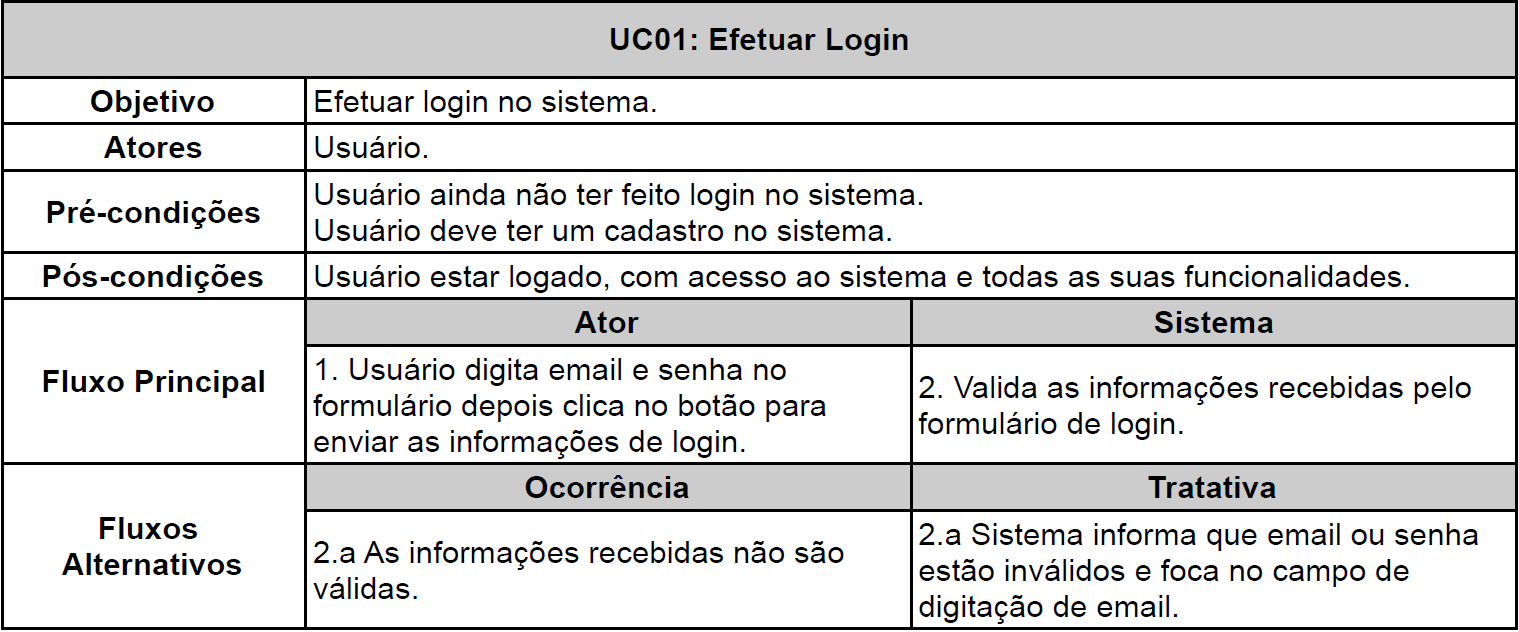
\includegraphics[width=1\textwidth]{./assets/apendices/UC01Admink}}% measure width
	    \begin{minipage}{\wd0}
		    \usebox0
		    \caption[]{UC01: Efetuar Login}
		    \label{fig:uc1-admink}
		    \fonte{o Autor}
	    \end{minipage}
    \end{figure}
    

    \begin{figure}[!htb]
	    \centering
	    \sbox0{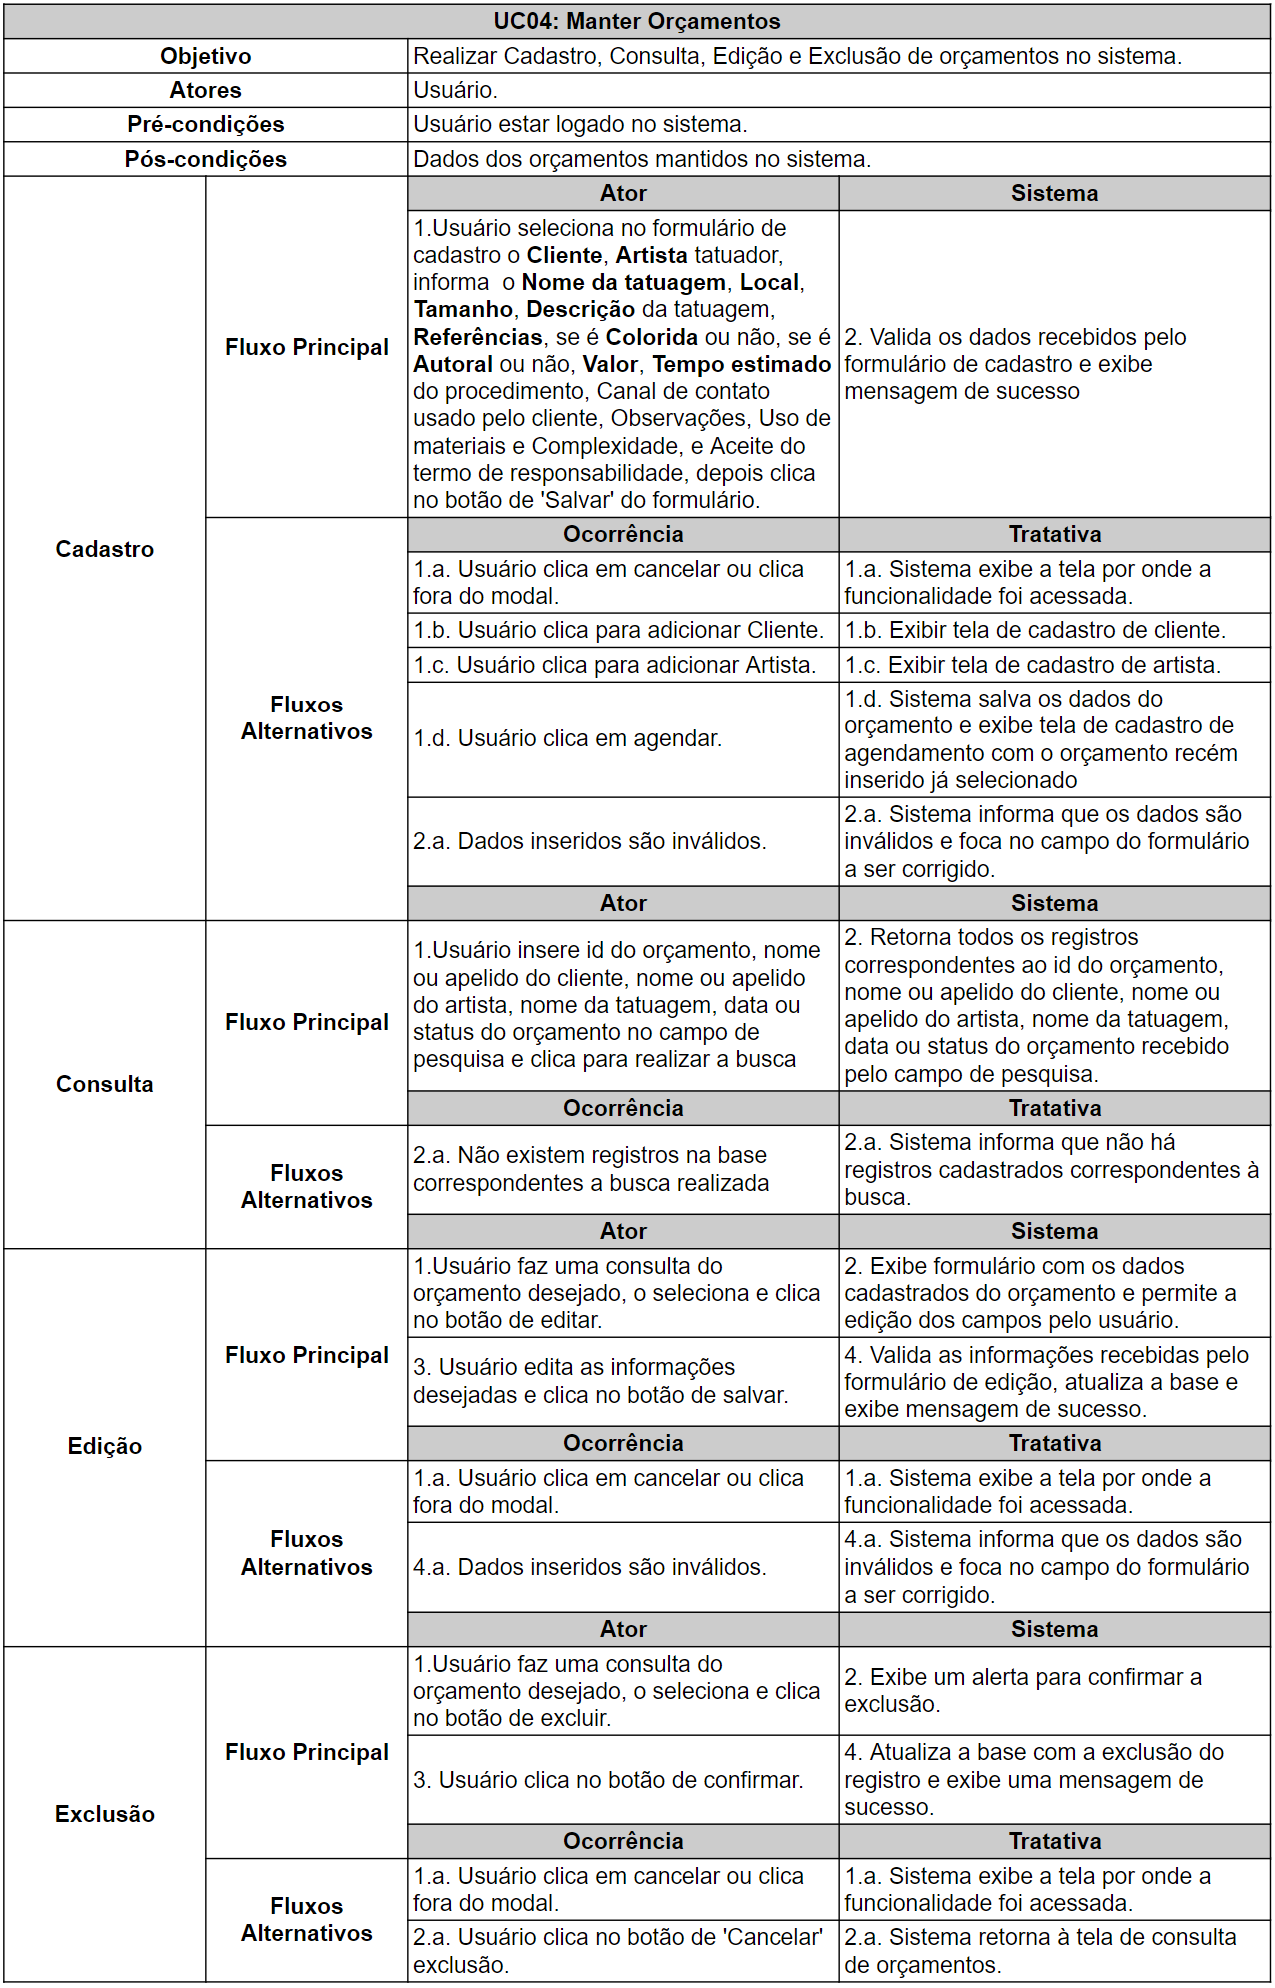
\includegraphics[width=1\textwidth]{./assets/apendices/UC04Admink}}% measure width
	    \begin{minipage}{\wd0}
		    \usebox0
		    \caption[]{UC04: Manter Orçamentos}
		    \label{fig:uc4-admink}
		    \fonte{o Autor}
	    \end{minipage}
    \end{figure}

\chapter{Plano de Testes do Sistema Admink}
\label{chap:apendiceB}

\setcounter{figure}{0}

    \begin{figure}[!htb]
	    \centering
	    \sbox0{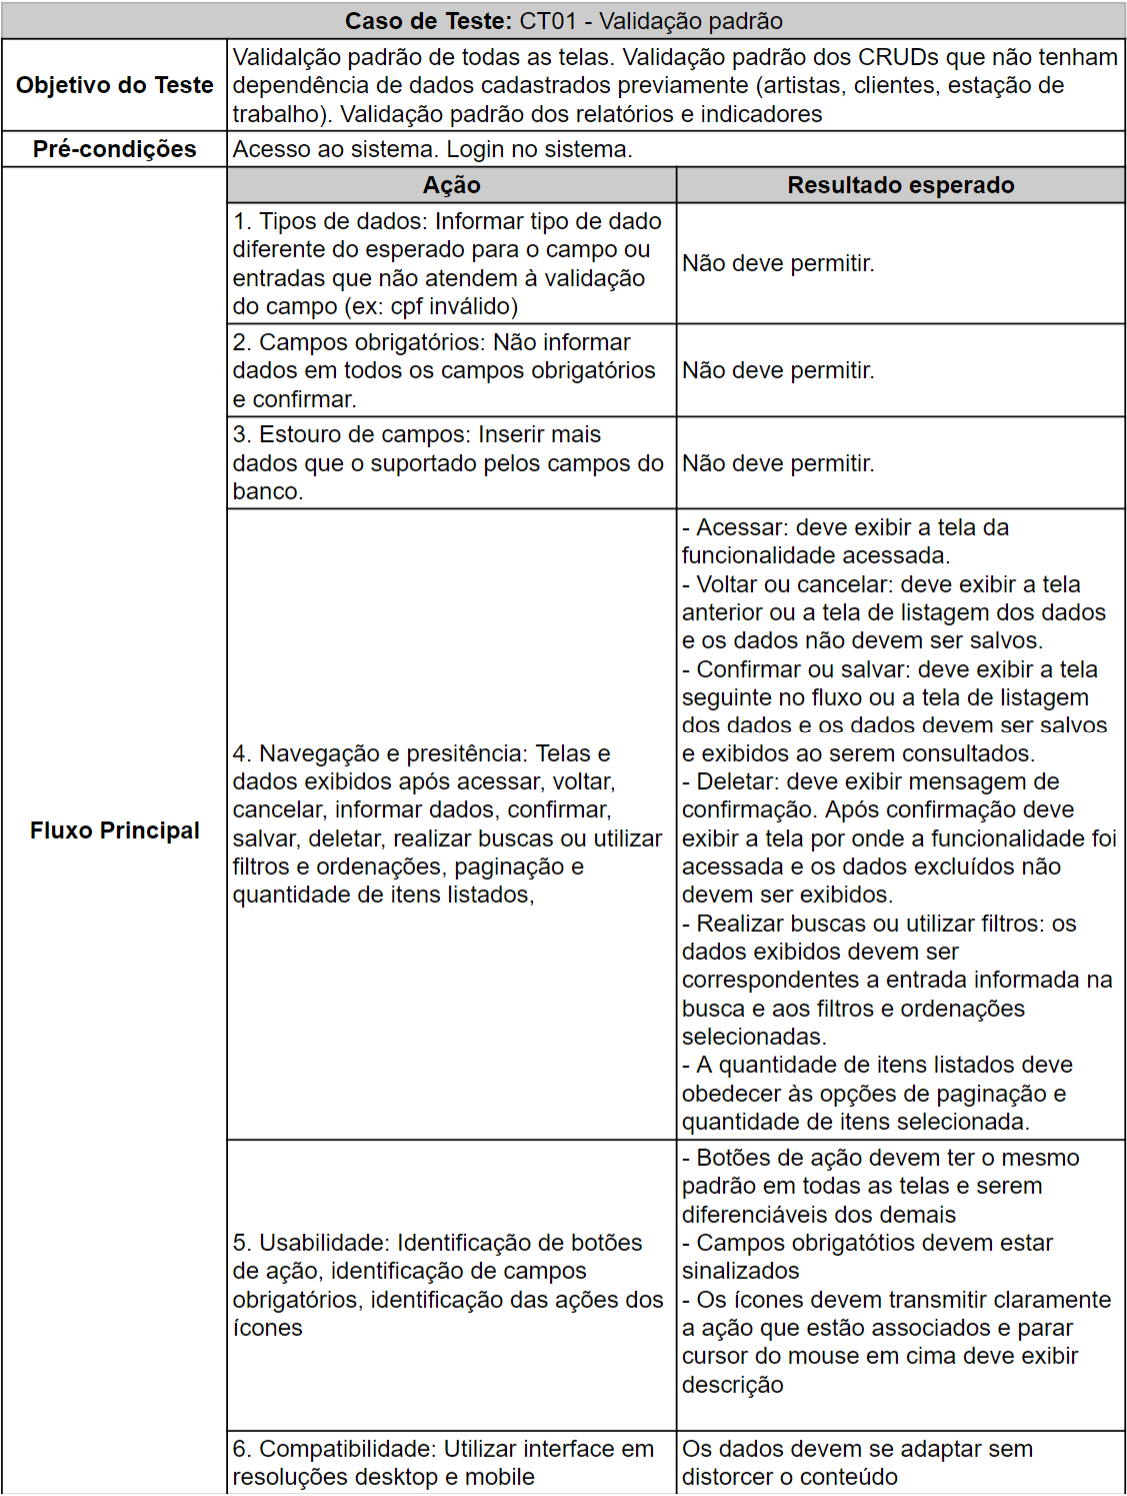
\includegraphics[width=1\textwidth]{./assets/apendices/CT01Admink}}% measure width
	    \begin{minipage}{\wd0}
		    \usebox0
		    \caption[]{TC01: Validação Padrão}
		    \label{fig:tc01-admink}
		    \fonte{o Autor}
	    \end{minipage}
    \end{figure}
    
    \begin{figure}[!htb]
	    \centering
	    \sbox0{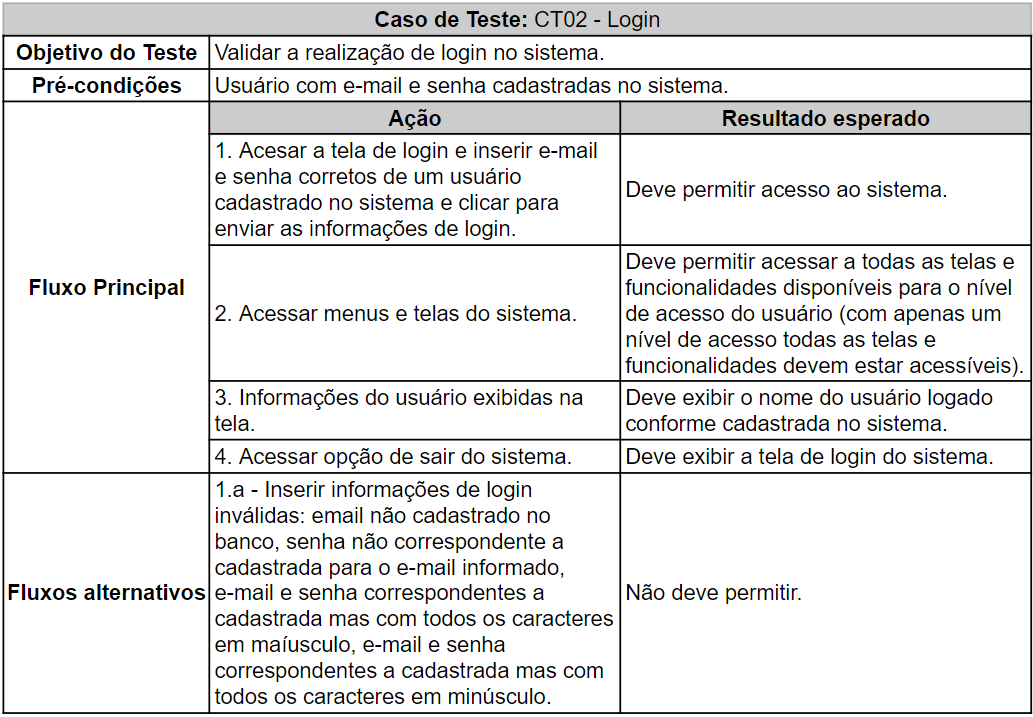
\includegraphics[width=1\textwidth]{./assets/apendices/CT02Admink}}% measure width
	    \begin{minipage}{\wd0}
		    \usebox0
		    \caption[]{TC02: Login}
		    \label{fig:tc02-admink}
		    \fonte{o Autor}
	    \end{minipage}
    \end{figure}
    
    \begin{figure}[!htb]
	    \centering
	    \sbox0{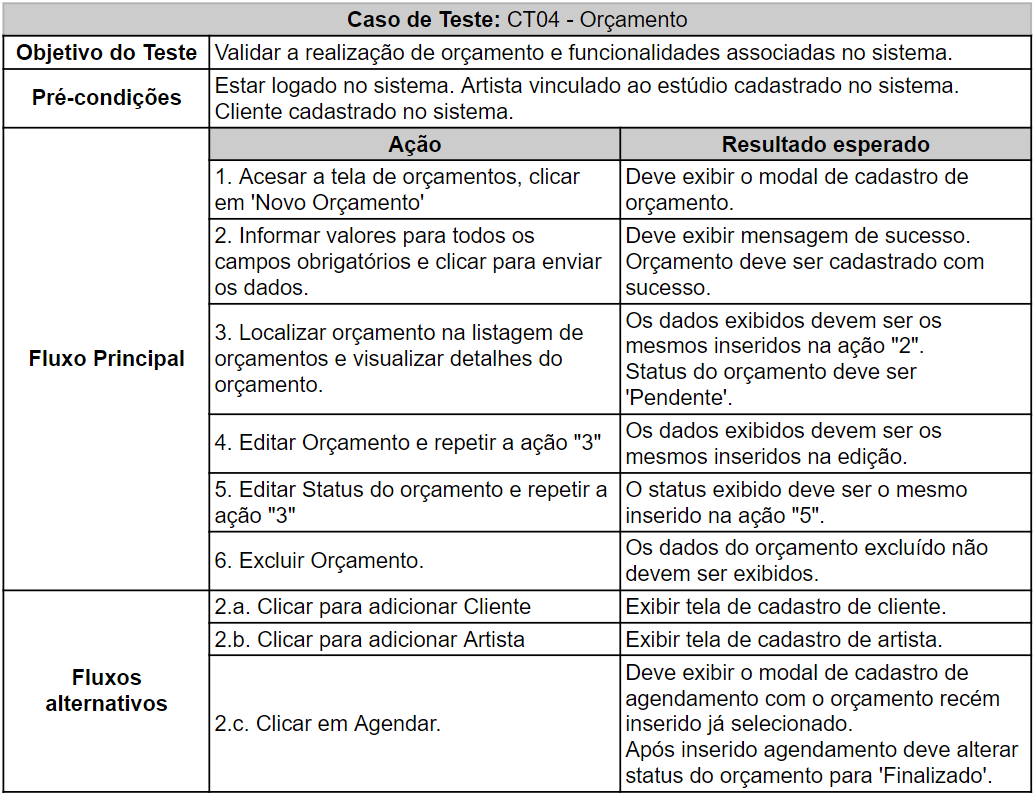
\includegraphics[width=1\textwidth]{./assets/apendices/CT04Admink}}% measure width
	    \begin{minipage}{\wd0}
		    \usebox0
		    \caption[]{TC04: Orçamento}
		    \label{fig:tc04-admink}
		    \fonte{o Autor}
	    \end{minipage}
    \end{figure}
    
\chapter{Scripts de Teste de Integração do Sistema Admink}
\label{chap:apendiceC}

\begin{lstlisting}[language=PHP, caption= Scripts de teste de Login, nolol,
label={code:LoginTest}]

<?php

namespace Tests\Integration\Login;

use Tests\TestCase;
use App\User;

class LoginTest extends TestCase
{

    public function teste1LoginComSucessoComEmailESenhaValidos()
    {
        $user = factory(User::class)->create();
        $response = $this->call('POST', '/login', ['email' => $user->email, 'password' => 'teste@123']);
        $response->assertStatus(302);
        $response->assertRedirect('/admin/home');
    }

    public function teste2LogincomFalhaComEmailInvalido()
    {
        $user = factory(User::class)->create();
        $response = $this->call('POST', '/login', ['email' => 'invalido@email.com', 'password' => 'teste@123']);
        $response->assertStatus(302);
        $response->assertRedirect('/');
    }

    public function teste3LogincomFalhaComEmailESenhaVazios()
    {
        $user = factory(User::class)->create();
        $response = $this->call('POST', '/login', ['email' => '', 'password' => '']);
        $response->assertStatus(302);
        $response->assertRedirect('/');
    }
    public function teste4LogincomFalhaComEmailESenhaNulos()
    {
        $user = factory(User::class)->create();
        $response = $this->call('POST', '/login', ['email' => null, 'password' => null]);
        $response->assertStatus(302);
        $response->assertRedirect('/');
    }

    public function teste5LogincomFalhaComSenhaIncorreta()
    {
        $user = factory(User::class)->create();
        $response = $this->call('POST', '/login', ['email' => $user->email, 'password' => 'wrongpassowrd']);
        $response->assertStatus(302);
        $response->assertRedirect('/');
    }
}
    
\end{lstlisting}

\fonte{o Autor}

\begin{lstlisting}[language=PHP, caption= Scripts de teste de Criação de Orçamentos, nolol,
label={code:CriacaoDeOrcamentoTest}]
<?php

namespace Tests\Integration\Orcamentos;

use Tests\TestCase;
use App\User;
use App\EstudioUsers;
use App\Estudio;
use App\Cliente;
use App\Artista;
use App\ArtistaEstudio;
use App\ClienteEstudio;


class CriacaoDeOrcamentoTest extends TestCase
{
    public function teste1CriacaoDeOrcamentoComSucessoDadosCorretos()
    {
        $user = factory(User::class)->create();
        $estudio = factory(Estudio::class)->create();
        factory(EstudioUsers::class)->create(['fk_users_id_users' => $user->id, 'fk_estudio_id_estudio' => $estudio->id_estudio]);
        $artista = factory(Artista::class)->create();
        $cliente = factory(Cliente::class)->create();
        factory(ArtistaEstudio::class)->create(['fk_artista_id_artista' => $artista->id_artista, 'fk_estudio_id_estudio' => $estudio->id_estudio]);
        factory(ClienteEstudio::class)->create(['fk_cliente_id_cliente' => $cliente->id_cliente, 'fk_estudio_id_estudio' => $estudio->id_estudio]);


        $response = $this->actingAs($user)
            ->post('/admin/orcamentos', [
                'cliente'               => $cliente->id_cliente,
                'artista'               => $artista->id_artista,
                'tatuagem_nome'         => 'Teste Orçamento',
                'tatuagem_local'        => 'Teste',
                'tatuagem_comprimento'  => 10,
                'tatuagem_largura'      => 10,
                'tatuagem_descricao'    => 'Teste Orçamento Criado com Sucesso!',
                'tatuagem_referencias'  => null,
                'canal_contato'         => null,
                'tempo_estimado'        => null,
                'valor'                 => null,
                'uso_materiais'         => null,
                'complexidade'          => null,
                'observacao'            => null
            ]);
        $response->assertStatus(302);
        $response->assertSessionHas('success_toastr', 'O orçamento foi cadastrado com sucesso!');
    }

    public function teste2CriacaoDeOrcamentoComFalhaDadosObrigatorioVazios()
    {
        $user = factory(User::class)->create();
        $estudio = factory(Estudio::class)->create();
        factory(EstudioUsers::class)->create(['fk_users_id_users' => $user->id, 'fk_estudio_id_estudio' => $estudio->id_estudio]);

        $response = $this->actingAs($user)
            ->post('/admin/orcamentos', [
                'cliente'               => null,
                'artista'               => null,
                'tatuagem_nome'         => '',
                'tatuagem_local'        => '',
                'tatuagem_comprimento'  => null,
                'tatuagem_largura'      => null,
                'tatuagem_descricao'    => '',
                'tatuagem_referencias'  => null,
                'canal_contato'         => null,
                'tempo_estimado'        => null,
                'valor'                 => null,
                'uso_materiais'         => null,
                'complexidade'          => null,
                'observacao'            => null
            ]);

        $response->assertStatus(302);
        $this->assertEquals(session('errors')->get('cliente')[0], 'O campo cliente é obrigatório.');
        $this->assertEquals(session('errors')->get('artista')[0], 'O campo artista é obrigatório.');
        $this->assertEquals(session('errors')->get('tatuagem_nome')[0], 'O campo tatuagem nome é obrigatório.');
        $this->assertEquals(session('errors')->get('tatuagem_local')[0], 'O campo tatuagem local é obrigatório.');
        $this->assertEquals(session('errors')->get('tatuagem_comprimento')[0], 'O campo tatuagem comprimento é obrigatório.');
        $this->assertEquals(session('errors')->get('tatuagem_largura')[0], 'O campo tatuagem largura é obrigatório.');
        $this->assertEquals(session('errors')->get('tatuagem_descricao')[0], 'O campo tatuagem descricao é obrigatório.');
    }

    public function teste3CriacaoDeOrcamentoComFalhaDadosComTamanhoMaiorQueOSuportado()
    {
        include  'TestStrings.php';
        $user = factory(User::class)->create();
        $estudio = factory(Estudio::class)->create();
        factory(EstudioUsers::class)->create(['fk_users_id_users' => $user->id, 'fk_estudio_id_estudio' => $estudio->id_estudio]);

        $response = $this->actingAs($user)
            ->post('/admin/orcamentos', [
                'cliente'               => 2147483648,
                'artista'               => 2147483648,
                'tatuagem_nome'         => 'String com 61 caracteres  TETESTETESTETESTETESTETESTETESTETES',
                'tatuagem_local'        => 'String com 61 caracteres  TETESTETESTETESTETESTETESTETESTETES',
                'tatuagem_comprimento'  => 201,
                'tatuagem_largura'      => 201,
                'tatuagem_descricao'    => 'String com 256 caracteres ESTETESTETESTETESTETESTETESTETESTETESTETESTETESTETESTETESTETESTETESTETESTETESTETESTETESTETESTETESTETESTETESTETESTETESTETESTETESTETESTETESTETESTETESTETESTETESTETESTETESTETESTETESTETESTETESTETESTETESTETESTETESTETESTETESTETESTETESTET',
                'tatuagem_referencias'  => $stringCom65536caracteres,
                'canal_contato'         => 2147483648,
                'tempo_estimado'        => '24:00:00',
                'valor'                 => 100000,
                'uso_materiais'         => 2147483648,
                'complexidade'          => 2147483648,
                'observacao'            => 'String com 256 caracteres ESTETESTETESTETESTETESTETESTETESTETESTETESTETESTETESTETESTETESTETESTETESTETESTETESTETESTETESTETESTETESTETESTETESTETESTETESTETESTETESTETESTETESTETESTETESTETESTETESTETESTETESTETESTETESTETESTETESTETESTETESTETESTETESTETESTETESTETESTET'
            ]);

        $response->assertStatus(302);
        $this->assertEquals(session('errors')->get('tatuagem_nome')[0], 'O campo tatuagem nome não pode ser superior a 60 caracteres.');
        $this->assertEquals(session('errors')->get('tatuagem_local')[0], 'O campo tatuagem local não pode ser superior a 60 caracteres.');
        $this->assertEquals(session('errors')->get('tatuagem_comprimento')[0], 'O campo tatuagem comprimento não pode ser superior a 200.');
        $this->assertEquals(session('errors')->get('tatuagem_largura')[0], 'O campo tatuagem largura não pode ser superior a 200.');
        $this->assertEquals(session('errors')->get('tatuagem_descricao')[0], 'O campo tatuagem descricao não pode ser superior a 255 caracteres.');
        $this->assertEquals(session('errors')->get('valor')[0], 'O valor do orçamento deve estar entre R$ 0,00 e R$ 99.999,99');
        $this->assertEquals(session('errors')->get('tempo_estimado')[0], 'O tempo estimado deve estar entre 00:00 e 23:59');
        $this->assertEquals(session('errors')->get('observacao')[0], 'O campo observacao não pode ser superior a 255 caracteres.');
    }

    public function teste4CriacaoDeOrcamentoComFalhaDadosComTiposDiferentesDoSuportado()
    {
        $user = factory(User::class)->create();
        $estudio = factory(Estudio::class)->create();
        factory(EstudioUsers::class)->create(['fk_users_id_users' => $user->id, 'fk_estudio_id_estudio' => $estudio->id_estudio]);

        $response = $this->actingAs($user)
            ->post('/admin/orcamentos', [
                'cliente'               => 'String ao invés de inteiro',
                'artista'               => 'String ao invés de inteiro',
                'tatuagem_nome'         => 73273,
                'tatuagem_local'        => 73273,
                'tatuagem_comprimento'  => 'String ao invés de inteiro',
                'tatuagem_largura'      => 'String ao invés de inteiro',
                'tatuagem_descricao'    => ['array ao invés', 'de string'],
                'tatuagem_referencias'  => 73273,
                'canal_contato'         => ['array ao invés', 'de string'],
                'tempo_estimado'        => 1643067873,
                'valor'                 => 'String ao invés de float',
                'uso_materiais'         => 'String ao invés de inteiro',
                'complexidade'          => 'String ao invés de inteiro',
                'observacao'            => 'String com 256 caracteres ESTETESTETESTETESTETESTETESTETESTETESTETESTETESTETESTETESTETESTETESTETESTETESTETESTETESTETESTETESTETESTETESTETESTETESTETESTETESTETESTETESTETESTETESTETESTETESTETESTETESTETESTETESTETESTETESTETESTETESTETESTETESTETESTETESTETESTETESTET'
            ]);

        $response->assertStatus(302);
        $this->assertEquals(session('errors')->get('tatuagem_nome')[0], 'O campo tatuagem nome deve ser uma string.');
        $this->assertEquals(session('errors')->get('tatuagem_local')[0], 'O campo tatuagem local deve ser uma string.');
        $this->assertEquals(session('errors')->get('tatuagem_comprimento')[0], 'O campo tatuagem comprimento deve ser um número.');
        $this->assertEquals(session('errors')->get('tatuagem_largura')[0], 'O campo tatuagem largura deve ser um número.');
        $this->assertEquals(session('errors')->get('tatuagem_descricao')[0], 'O campo tatuagem descricao deve ser uma string.');
        $this->assertEquals(session('errors')->get('valor')[0], 'O valor do orçamento deve estar entre R$ 0,00 e R$ 99.999,99');
        $this->assertEquals(session('errors')->get('tempo_estimado')[0], 'O tempo estimado deve estar entre 00:00 e 23:59');
        $this->assertEquals(session('errors')->get('observacao')[0], 'O campo observacao não pode ser superior a 255 caracteres.');
    }
}
    
\end{lstlisting}

\fonte{o Autor}

\begin{lstlisting}[language=PHP, caption= Scripts de teste de Edição de Orçamentos, nolol,
label={code:EdicaoDeOrcamentoTest}]
<?php

namespace Tests\Integration\Orcamentos;

use Tests\TestCase;
use App\User;
use App\EstudioUsers;
use App\Orcamento;
use App\Estudio;
use App\Cliente;
use App\Artista;
use App\ArtistaEstudio;
use App\ClienteEstudio;

class EdicaoDeOrcamentosTest extends TestCase
{

    public function teste1EdicaoDeOrcamentoComSucessoSemDadosDeTatuador()
    {
        $user = factory(User::class)->create();
        $estudio = factory(Estudio::class)->create();
        factory(EstudioUsers::class)->create(['fk_users_id_users' => $user->id, 'fk_estudio_id_estudio' => $estudio->id_estudio]);
        $artista = factory(Artista::class)->create();
        $cliente = factory(Cliente::class)->create();
        factory(ArtistaEstudio::class)->create(['fk_artista_id_artista' => $artista->id_artista, 'fk_estudio_id_estudio' => $estudio->id_estudio]);
        factory(ClienteEstudio::class)->create(['fk_cliente_id_cliente' => $cliente->id_cliente, 'fk_estudio_id_estudio' => $estudio->id_estudio]);
        $orcamento = factory(Orcamento::class)->create(['fk_cliente_id_cliente' => $cliente->id_cliente, 'fk_artista_id_artista' => $artista->id_artista, 'fk_estudio_id_estudio' => $estudio->id_estudio, 'fk_orcamento_status_id_orcamento_status' => 1]);

        $response = $this->actingAs($user)
            ->post('/admin/orcamentos/' . $orcamento->id_orcamento, [
                '_method'               => 'PUT',
                'cliente'               => $cliente->id_cliente,
                'artista'               => $artista->id_artista,
                'tatuagem_nome'         => 'Teste Edição Orçamento',
                'tatuagem_local'        => 'Teste Edição Orçamento',
                'tatuagem_comprimento'  => 13,
                'tatuagem_largura'      => 13,
                'tatuagem_descricao'    => 'Teste Orçamento Editado com Sucesso!',
                'tatuagem_referencias'  => 'testeedicaoorcamento.com.br',
                'canal_contato'         => 'Teste Edição',
                'tempo_estimado'        => null,
                'valor'                 => null,
                'uso_materiais'         => null,
                'complexidade'          => null,
                'observacao'            => null
            ]);
        $response->assertStatus(302);
        $response->assertSessionHas('success_toastr', 'O orçamento foi atualizado com sucesso!');
    }

    public function teste2EdicaoDeOrcamentoComSucessoComDadosDeTatuador()
    {
        $user = factory(User::class)->create();
        $estudio = factory(Estudio::class)->create();
        factory(EstudioUsers::class)->create(['fk_users_id_users' => $user->id, 'fk_estudio_id_estudio' => $estudio->id_estudio]);
        $artista = factory(Artista::class)->create();
        $cliente = factory(Cliente::class)->create();
        factory(ArtistaEstudio::class)->create(['fk_artista_id_artista' => $artista->id_artista, 'fk_estudio_id_estudio' => $estudio->id_estudio]);
        factory(ClienteEstudio::class)->create(['fk_cliente_id_cliente' => $cliente->id_cliente, 'fk_estudio_id_estudio' => $estudio->id_estudio]);
        $orcamento = factory(Orcamento::class)->create(['fk_cliente_id_cliente' => $cliente->id_cliente, 'fk_artista_id_artista' => $artista->id_artista, 'fk_estudio_id_estudio' => $estudio->id_estudio, 'fk_orcamento_status_id_orcamento_status' => 1]);

        $response = $this->actingAs($user)
            ->post('/admin/orcamentos/' . $orcamento->id_orcamento, [
                '_method'               => 'PUT',
                'cliente'               => $cliente->id_cliente,
                'artista'               => $artista->id_artista,
                'tatuagem_nome'         => 'Teste Edição Orçamento',
                'tatuagem_local'        => 'Teste Edição Orçamento',
                'tatuagem_comprimento'  => 13,
                'tatuagem_largura'      => 13,
                'tatuagem_descricao'    => 'Teste Orçamento Editado com Sucesso!',
                'tatuagem_referencias'  => 'testeedicaoorcamento.com.br',
                'canal_contato'         => 'Teste Edição',
                'tempo_estimado'        => '03:00',
                'valor'                 => '13,00',
                'uso_materiais'         => 1,
                'complexidade'          => 1,
                'observacao'            => 'Teste Edição de Orçamento com sucesso com dados de tatuador!'
            ]);
        $response->assertStatus(302);
        $response->assertSessionHas('success_toastr', 'O orçamento foi atualizado com sucesso!');
    }

    public function teste3EdicaoDeOrcamentoComFalhaDadosObrigatoriosVazios()
    {
        $user = factory(User::class)->create();
        $estudio = factory(Estudio::class)->create();
        factory(EstudioUsers::class)->create(['fk_users_id_users' => $user->id, 'fk_estudio_id_estudio' => $estudio->id_estudio]);
        $artista = factory(Artista::class)->create();
        $cliente = factory(Cliente::class)->create();
        factory(ArtistaEstudio::class)->create(['fk_artista_id_artista' => $artista->id_artista, 'fk_estudio_id_estudio' => $estudio->id_estudio]);
        factory(ClienteEstudio::class)->create(['fk_cliente_id_cliente' => $cliente->id_cliente, 'fk_estudio_id_estudio' => $estudio->id_estudio]);
        $orcamento = factory(Orcamento::class)->create(['fk_cliente_id_cliente' => $cliente->id_cliente, 'fk_artista_id_artista' => $artista->id_artista, 'fk_estudio_id_estudio' => $estudio->id_estudio, 'fk_orcamento_status_id_orcamento_status' => 1]);

        $response = $this->actingAs($user)
            ->post('/admin/orcamentos/' . $orcamento->id_orcamento, [
                '_method'               => 'PUT',
                'cliente'               => null,
                'artista'               => null,
                'tatuagem_nome'         => '',
                'tatuagem_local'        => '',
                'tatuagem_comprimento'  => null,
                'tatuagem_largura'      => null,
                'tatuagem_descricao'    => '',
                'tatuagem_referencias'  => null,
                'canal_contato'         => null,
                'tempo_estimado'        => null,
                'valor'                 => null,
                'uso_materiais'         => null,
                'complexidade'          => null,
                'observacao'            => null
            ]);
        $response->assertStatus(302);
        $this->assertEquals(session('errors')->get('cliente')[0], 'O campo cliente é obrigatório.');
        $this->assertEquals(session('errors')->get('artista')[0], 'O campo artista é obrigatório.');
        $this->assertEquals(session('errors')->get('tatuagem_nome')[0], 'O campo tatuagem nome é obrigatório.');
        $this->assertEquals(session('errors')->get('tatuagem_local')[0], 'O campo tatuagem local é obrigatório.');
        $this->assertEquals(session('errors')->get('tatuagem_comprimento')[0], 'O campo tatuagem comprimento é obrigatório.');
        $this->assertEquals(session('errors')->get('tatuagem_largura')[0], 'O campo tatuagem largura é obrigatório.');
        $this->assertEquals(session('errors')->get('tatuagem_descricao')[0], 'O campo tatuagem descricao é obrigatório.');
    }

    public function teste4EdicaoDeOrcamentoComFalhaDadosComTamanhoMaiorQueOSuportado()
    {   
        include  'TestStrings.php';
        $user = factory(User::class)->create();
        $estudio = factory(Estudio::class)->create();
        factory(EstudioUsers::class)->create(['fk_users_id_users' => $user->id, 'fk_estudio_id_estudio' => $estudio->id_estudio]);
        $artista = factory(Artista::class)->create();
        $cliente = factory(Cliente::class)->create();
        factory(ArtistaEstudio::class)->create(['fk_artista_id_artista' => $artista->id_artista, 'fk_estudio_id_estudio' => $estudio->id_estudio]);
        factory(ClienteEstudio::class)->create(['fk_cliente_id_cliente' => $cliente->id_cliente, 'fk_estudio_id_estudio' => $estudio->id_estudio]);
        $orcamento = factory(Orcamento::class)->create(['fk_cliente_id_cliente' => $cliente->id_cliente, 'fk_artista_id_artista' => $artista->id_artista, 'fk_estudio_id_estudio' => $estudio->id_estudio, 'fk_orcamento_status_id_orcamento_status' => 1]);
        
        $response = $this->actingAs($user)
            ->post('/admin/orcamentos/' . $orcamento->id_orcamento, [
                '_method'               => 'PUT',
                'cliente'               => 2147483648,
                'artista'               => 2147483648,
                'tatuagem_nome'         => $stringCom61Caracteres,
                'tatuagem_local'        => $stringCom61Caracteres,
                'tatuagem_comprimento'  => 201,
                'tatuagem_largura'      => 201,
                'tatuagem_descricao'    => $stringCom256Caracteres,
                'tatuagem_referencias'  => $stringCom65536Caracteres,
                'canal_contato'         => 2147483648,
                'tempo_estimado'        => '24:00:00',
                'valor'                 => '100.000,00',
                'uso_materiais'         => 2147483648,
                'complexidade'          => 2147483648,
                'observacao'            => $stringCom256Caracteres
            ]);

        $response->assertStatus(302);
        $this->assertEquals(session('errors')->get('tatuagem_nome')[0], 'O campo tatuagem nome não pode ser superior a 60 caracteres.');
        $this->assertEquals(session('errors')->get('tatuagem_local')[0], 'O campo tatuagem local não pode ser superior a 60 caracteres.');
        $this->assertEquals(session('errors')->get('tatuagem_comprimento')[0], 'O campo tatuagem comprimento não pode ser superior a 200.');
        $this->assertEquals(session('errors')->get('tatuagem_largura')[0], 'O campo tatuagem largura não pode ser superior a 200.');
        $this->assertEquals(session('errors')->get('tatuagem_descricao')[0], 'O campo tatuagem descricao não pode ser superior a 255 caracteres.');
        $this->assertEquals(session('errors')->get('valor')[0], 'O campo valor tem um formato inválido.');
        $this->assertEquals(session('errors')->get('tempo_estimado')[0], 'O campo tempo estimado tem um formato inválido.');
        $this->assertEquals(session('errors')->get('observacao')[0], 'O campo observacao não pode ser superior a 255 caracteres.');
    }

    public function teste5EdicaoDeOrcamentoComFalhaDadosComTiposDiferentesDoSuportado()
    {
        include  'TestStrings.php';
        $user = factory(User::class)->create();
        $estudio = factory(Estudio::class)->create();
        factory(EstudioUsers::class)->create(['fk_users_id_users' => $user->id, 'fk_estudio_id_estudio' => $estudio->id_estudio]);
        $artista = factory(Artista::class)->create();
        $cliente = factory(Cliente::class)->create();
        factory(ArtistaEstudio::class)->create(['fk_artista_id_artista' => $artista->id_artista, 'fk_estudio_id_estudio' => $estudio->id_estudio]);
        factory(ClienteEstudio::class)->create(['fk_cliente_id_cliente' => $cliente->id_cliente, 'fk_estudio_id_estudio' => $estudio->id_estudio]);
        $orcamento = factory(Orcamento::class)->create(['fk_cliente_id_cliente' => $cliente->id_cliente, 'fk_artista_id_artista' => $artista->id_artista, 'fk_estudio_id_estudio' => $estudio->id_estudio, 'fk_orcamento_status_id_orcamento_status' => 1]);

        $response = $this->actingAs($user)
            ->post('/admin/orcamentos/' . $orcamento->id_orcamento, [
                '_method'               => 'PUT',
                'cliente'               => 'String ao invés de inteiro',
                'artista'               => 'String ao invés de inteiro',
                'tatuagem_nome'         => 73273,
                'tatuagem_local'        => 73273,
                'tatuagem_comprimento'  => 'String ao invés de inteiro',
                'tatuagem_largura'      => 'String ao invés de inteiro',
                'tatuagem_descricao'    => ['array ao invés', 'de string'],
                'tatuagem_referencias'  => 73273,
                'canal_contato'         => ['array ao invés', 'de string'],
                'tempo_estimado'        => 1643067873,
                'valor'                 => 100000.00,
                'uso_materiais'         => 'String ao invés de inteiro',
                'complexidade'          => 'String ao invés de inteiro',
                'observacao'            => $stringCom256Caracteres
            ]);
        $response->assertStatus(302);
        $this->assertEquals(session('errors')->get('tatuagem_nome')[0], 'O campo tatuagem nome deve ser uma string.');
        $this->assertEquals(session('errors')->get('tatuagem_local')[0], 'O campo tatuagem local deve ser uma string.');
        $this->assertEquals(session('errors')->get('tatuagem_comprimento')[0], 'O campo tatuagem comprimento deve ser um número.');
        $this->assertEquals(session('errors')->get('tatuagem_largura')[0], 'O campo tatuagem largura deve ser um número.');
        $this->assertEquals(session('errors')->get('tatuagem_descricao')[0], 'O campo tatuagem descricao deve ser uma string.');
        $this->assertEquals(session('errors')->get('valor')[0], 'O campo valor tem um formato inválido.');
        $this->assertEquals(session('errors')->get('tempo_estimado')[0], 'O campo tempo estimado tem um formato inválido.');
        $this->assertEquals(session('errors')->get('observacao')[0], 'O campo observacao não pode ser superior a 255 caracteres.');
    }
}
\end{lstlisting}

\fonte{o Autor}

\begin{lstlisting}[language=PHP, caption= Scripts de teste de Listagem e Deleção de Orçamentos, nolol,
label={code:ListagemEDelecaoDeOrcamentosTest}]
<?php

namespace Tests\Integration\Orcamentos;

use Tests\TestCase;
use App\User;
use App\EstudioUsers;
use App\Orcamento;
use App\Estudio;
use App\Cliente;
use App\Artista;
use App\ArtistaEstudio;
use App\ClienteEstudio;
use App\Estacao;
use App\Agendamento;

class ListagemEDelecaoDeOrcamentosTest extends TestCase
{

    public function teste1ListagemDeOrcamentosComSucesso()
    {
        $user = factory(User::class)->create();
        $estudio = factory(Estudio::class)->create();
        factory(EstudioUsers::class)->create(['fk_users_id_users' => $user->id, 'fk_estudio_id_estudio' => $estudio->id_estudio]);
        $artista = factory(Artista::class)->create();
        $cliente = factory(Cliente::class)->create();
        factory(ArtistaEstudio::class)->create(['fk_artista_id_artista' => $artista->id_artista, 'fk_estudio_id_estudio' => $estudio->id_estudio]);
        factory(ClienteEstudio::class)->create(['fk_cliente_id_cliente' => $cliente->id_cliente, 'fk_estudio_id_estudio' => $estudio->id_estudio]);
        $orcamento = factory(Orcamento::class)->create(['fk_cliente_id_cliente' => $cliente->id_cliente, 'fk_artista_id_artista' => $artista->id_artista, 'fk_estudio_id_estudio' => $estudio->id_estudio, 'fk_orcamento_status_id_orcamento_status' => 1]);
        $orcamento2 = factory(Orcamento::class)->create(['fk_cliente_id_cliente' => $cliente->id_cliente, 'fk_artista_id_artista' => $artista->id_artista, 'fk_estudio_id_estudio' => $estudio->id_estudio, 'fk_orcamento_status_id_orcamento_status' => 1]);

        $response = $this->actingAs($user)
            ->get('/admin/orcamentos');

        $response->assertStatus(200);
        $response->assertSee('<td class="align-middle">' . $orcamento->tatuagem_nome . '</td>', $escaped = false);
        $response->assertSee('<td class="align-middle">#' . str_pad($orcamento->id_orcamento, 5, '0', STR_PAD_LEFT) . '</td>', $escaped = false);
        $response->assertSee('<td class="align-middle">' . $orcamento2->tatuagem_nome . '</td>', $escaped = false);
        $response->assertSee('<td class="align-middle">#' . str_pad($orcamento2->id_orcamento, 5, '0', STR_PAD_LEFT) . '</td>', $escaped = false);
    }

    public function teste2ExclusaoDeOrcamentoNaoAgendadoComSucesso()
    {
        $user = factory(User::class)->create();
        $estudio = factory(Estudio::class)->create();
        factory(EstudioUsers::class)->create(['fk_users_id_users' => $user->id, 'fk_estudio_id_estudio' => $estudio->id_estudio]);
        $artista = factory(Artista::class)->create();
        $cliente = factory(Cliente::class)->create();
        factory(ArtistaEstudio::class)->create(['fk_artista_id_artista' => $artista->id_artista, 'fk_estudio_id_estudio' => $estudio->id_estudio]);
        factory(ClienteEstudio::class)->create(['fk_cliente_id_cliente' => $cliente->id_cliente, 'fk_estudio_id_estudio' => $estudio->id_estudio]);
        $orcamento = factory(Orcamento::class)->create(['fk_cliente_id_cliente' => $cliente->id_cliente, 'fk_artista_id_artista' => $artista->id_artista, 'fk_estudio_id_estudio' => $estudio->id_estudio, 'fk_orcamento_status_id_orcamento_status' => 1]);

        $response = $this->actingAs($user)
            ->post('/admin/orcamentos/' . $orcamento->id_orcamento, [
                '_method'   => 'DELETE'
            ]);
        $response->assertStatus(302);
        $response->assertSessionHas('success_toastr',  'O orçamento foi excluído com sucesso!');
    }

    public function teste3ExclusaoDeOrcamentoAgendadoComSucesso()
    {
        $user = factory(User::class)->create();
        $estudio = factory(Estudio::class)->create();
        factory(EstudioUsers::class)->create(['fk_users_id_users' => $user->id, 'fk_estudio_id_estudio' => $estudio->id_estudio]);
        $artista = factory(Artista::class)->create();
        $cliente = factory(Cliente::class)->create();
        factory(ArtistaEstudio::class)->create(['fk_artista_id_artista' => $artista->id_artista, 'fk_estudio_id_estudio' => $estudio->id_estudio]);
        factory(ClienteEstudio::class)->create(['fk_cliente_id_cliente' => $cliente->id_cliente, 'fk_estudio_id_estudio' => $estudio->id_estudio]);
        $orcamento = factory(Orcamento::class)->create(['fk_cliente_id_cliente' => $cliente->id_cliente, 'fk_artista_id_artista' => $artista->id_artista, 'fk_estudio_id_estudio' => $estudio->id_estudio, 'fk_orcamento_status_id_orcamento_status' => 2, 'tempo_estimado' => '  02:00:00', 'valor' => 500.00, 'fk_uso_materiais_id_uso_materiais' => 1, 'fk_complexidade_id_complexidade' => 1, 'observacao' => 'teste3ExclusaoDeOrcamentoAgendadoComSucesso']);
        $estacao = factory(Estacao::class)->create(['fk_estudio_id_estudio' => $estudio->id_estudio]);
        factory(Agendamento::class)->create(['fk_orcamento_id_orcamento' => $orcamento->id_orcamento, 'fk_estacao_id_estacao' => $estacao->id_estacao, 'fk_agendamento_status_id_agendamento_status' => 1]);
        $orcamento->fk_orcamento_status_id_orcamento_status = 3;
        $orcamento->save();

        $response = $this->actingAs($user)
            ->post('/admin/orcamentos/' . $orcamento->id_orcamento, [
                '_method'   => 'DELETE'
            ]);
        $response->assertStatus(302);
        $response->assertSessionHas('success_toastr',  'O orçamento foi excluído com sucesso!');
    }
}
\end{lstlisting}

\fonte{o Autor}

\end{apendicesenv}





             			   % Apêndices
%% ANEXO------------------------------------------------------------------------

\begin{anexosenv}
\partanexos

% Primeiro anexo---------------------------------------------------------------
\chapter{Nome do anexo}     % edite para alterar o título deste anexo
\label{chap:anexoA}

% Novo anexo-------------------------------------------------------------------
\chapter{Nome do outro anexo}
\label{chap:anexoB}


\end{anexosenv}
               			   % Anexos

\end{document}
